% !TEX encoding = UTF-8 Unicode
\documentclass{article}
%\documentclass[12pt,reqno]{amsart}
\usepackage[russian]{babel}
\usepackage[utf8]{inputenc}
%\usepackage[dvips]{graphicx,graphics}
\usepackage{graphicx}
\usepackage{euscript}
\usepackage{graphics}
%\usepackage{russcorr}
\usepackage[active]{srcltx} % SRC Specials: DVI [Inverse] Search
\usepackage{amssymb,amsmath,amsthm,amsfonts}
\usepackage{amsopn}
\newtheorem{cor}{Следствие}
\newtheorem{lem}{Лемма}
\newtheorem{thm}{Теорема}
\newtheorem{prop}{Предложение}
\newtheorem*{thm_pres}{Теорема}
\theoremstyle{definition}
\newtheorem{defn}{Определение}
\newtheorem{defneq}{Эквивалентное определение}
\theoremstyle{remark}
\newtheorem*{rem}{Замечание}
\newtheorem*{deff}{Обозначение}
\usepackage{verbatim}
\usepackage{listings}
\usepackage{hyperref}
\usepackage{color}

\definecolor{dkgreen}{rgb}{0,0.5,0}
\definecolor{gray}{rgb}{0.5,0.5,0.5}
\definecolor{mauve}{rgb}{0.58,0,0.52}

\lstset{frame=tb,
  language=Java,
  aboveskip=3mm,
  belowskip=3mm,
  showstringspaces=false,
  columns=flexible,
  basicstyle={\small\ttfamily},
  numbers=none,
  numberstyle=\tiny\color{gray},
  keywordstyle=\color{blue},
  commentstyle=\color{dkgreen},
  stringstyle=\color{mauve},
  breaklines=true,
  breakatwhitespace=true,
  tabsize=3
}

\newcommand{\sug}[1]{\rule[-2mm]{0.4pt}{5mm}_{\,{#1}}}
\newcommand{\gen} {$GE^+_n(\mathbf{R}[x])\ $}
\newcommand{\genn} {$GE^+_2(\mathbf{R}[x])\ $}
\newcommand{\gn} {$G_n(\mathbf{R})\ $}
\newcommand{\gln} {$GL_n(\mathbf{R}[x])\ $}
\newcommand{\p} {\mathbf{P}}
\newcommand{\peq} {$\mathcal{P}$}
\newcommand{\po} {$\mathcal{P}_0$}
\newcommand{\ff} {$\mathbf{R}\ $}
\newcommand{\fx} {\mathbf{R}[x]}
\newcommand{\fp} {\mathbf{R_+}}
\newcommand{\fxp} {\mathbf{R_+}[x]}
\newcommand{\zx} {\mathbb{Z}[x]}
\newcommand{\zxp} {\mathbb{Z_+}[x]}
\newcommand{\basering} {$\mathbf{F}$}
\newcommand{\lfrac} [2] {\displaystyle \frac{#1}{#2}}
\newcommand{\brsum} [3] {\displaystyle \sum \limits_{#1}^{#2} \left( #3\right)}
\newcommand{\lsum} [2] {\displaystyle \sum \limits_{#1}^{#2}}
\newcommand{\br} [1] {\left( #1 \right)}
\newcommand{\tab} {\mbox{             } \quad }
\usepackage{a4wide}

\usepackage{verbatim}
\usepackage{hyperref}
\hypersetup{
    colorlinks,
    citecolor=black,
    filecolor=black,
    linkcolor=blue,
    urlcolor=blue
}
\setcounter{secnumdepth}{0}


\begin{document}
\section*{Отчет по первому практическому заданию}
\section*{Царькова Анастасия}

Формулы для градиента и гессиана функции логистической регрессии:

$$
f(x) = \lfrac{1}{m} \sum_{i = 1}^m \ln(1 + \exp(-b_ia_i^Tx)) + \lfrac{\lambda}{2} \|x\|_2^2 = \lfrac{1}{m} \ln(1 + \exp(-b * Ax)) + \lfrac{\lambda}{2} x^Tx
$$

$$
\nabla f(x) = -\lfrac{1}{m} A^T \left(b * \left(\lfrac{1}{1 - \exp(b * Ax)} \right)\right) + \lambda x = -\lfrac{1}{m} A^T \left(b * Expit(-b * Ax)\right) + \lambda x
$$

$$
\nabla^2 f(x) = \lfrac{1}{m} A^T Diag\left(\left(1 - \left(\lfrac{1}{1 - \exp(b * Ax)} \right)\right) * \left(\lfrac{1}{1 - \exp(b * Ax)} \right)\right)A + \lambda I =
$$

$$
= \lfrac{1}{m} A^T Diag\left(1 - Expit(b * Ax)\right) * \left(Expit(-b * Ax)\right)A + \lambda I
$$

\section{Первый эксперимент.}

Зависимость поведения метода от обусловденности функции.

В данном эксперименте предлагается проанализировать траекторию градиентого спуска в зависимости от:

1. Обусловленности функции

2. Выбора начальной точки

3. Стратегии выбора шага



Сравнивая графики с линиями уровня функции и траекториями методов.



Зададим объекты на которых будем сравнивать поведения методов:

1. Функции --  двемерные квадратичные функции с d нулю(для простоты) $f(x) = x^TAx + bx = x^TAx$.

$$
M_1 =
\begin{pmatrix}
1 &	0\\
0 &	2
\end{pmatrix}\ M_2 =
\begin{pmatrix}
1 &	0\\
0 &	60
\end{pmatrix}
$$


2. Начальные точки

$$
x_1 =
\begin{pmatrix}
1 \\
1
\end{pmatrix}\ x_2 =
\begin{pmatrix}
20 \\
30
\end{pmatrix}
$$

3. Cтратегии выбора шага: Armijo, Wolfe, Constant\\


Результаты эксперимента:\\


$\bullet$ Constant\\

Видно что метод работает не очень хорошо. Делает слишком много шагов, но не слишком чувствителек к выбору начальной точки.

Более того крайне чувствителен к обусловленности функции, на $M_2$ метод возвращает $computational_error$, поэтому я взяла вместо нее
$
M =\begin{pmatrix}1 &	0\\ 0 &	10
\end{pmatrix}
$
и все равно получила $iterations_exceeded$, но полученные графики очень показательны. Кажется что метот вряд ли сойдется при увеличениии числа итераций.


\begin{center}
\begin{tabular}{cc}
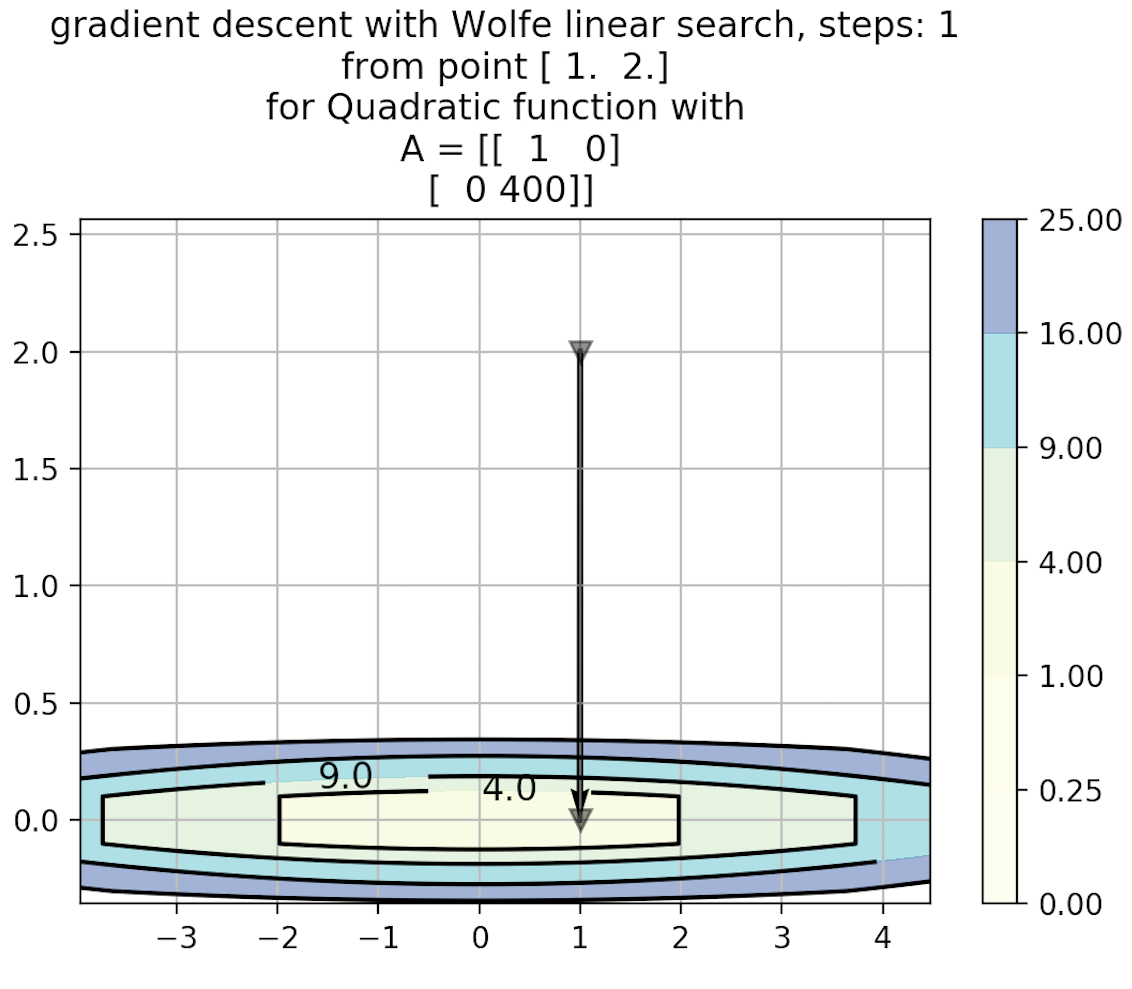
\includegraphics[width=0.49\linewidth]{15.png} &
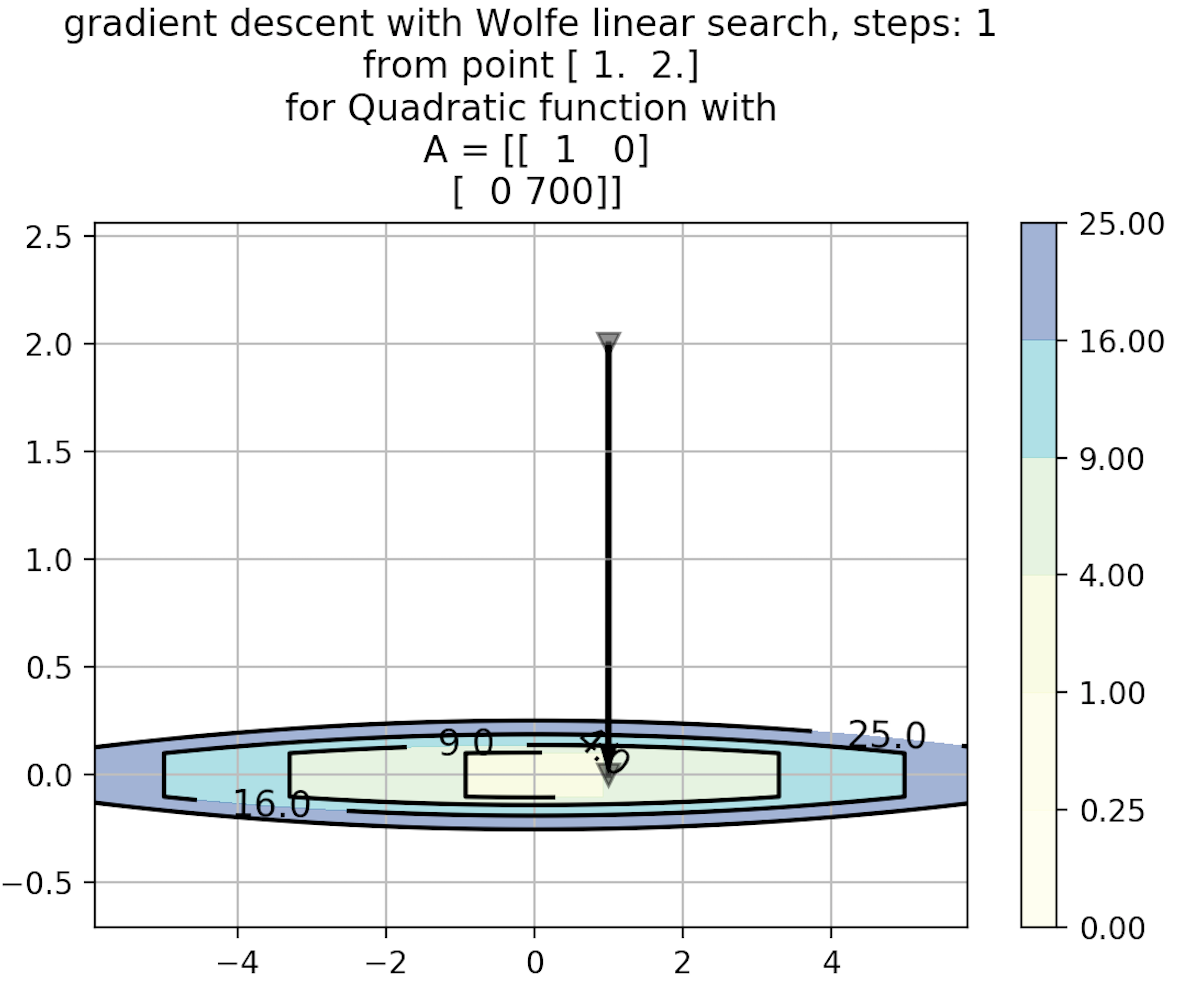
\includegraphics[width=0.49\linewidth]{16.png} \\
 a)$M_1,\ x_1$ & b)$M_1,\ x_2$\\
\end{tabular}
\end{center}
\begin{center}
\begin{tabular}{cc}
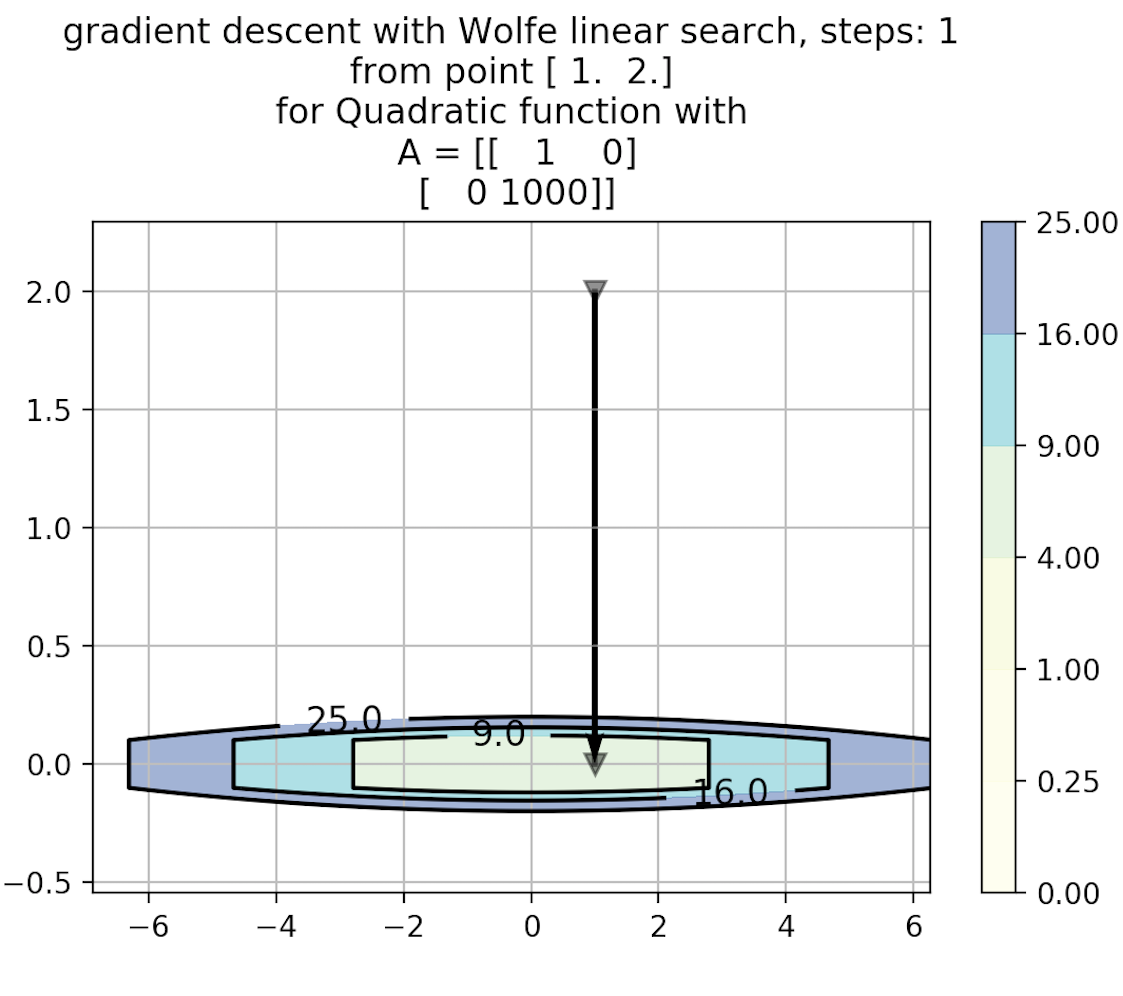
\includegraphics[width=0.49\linewidth]{17.png} &
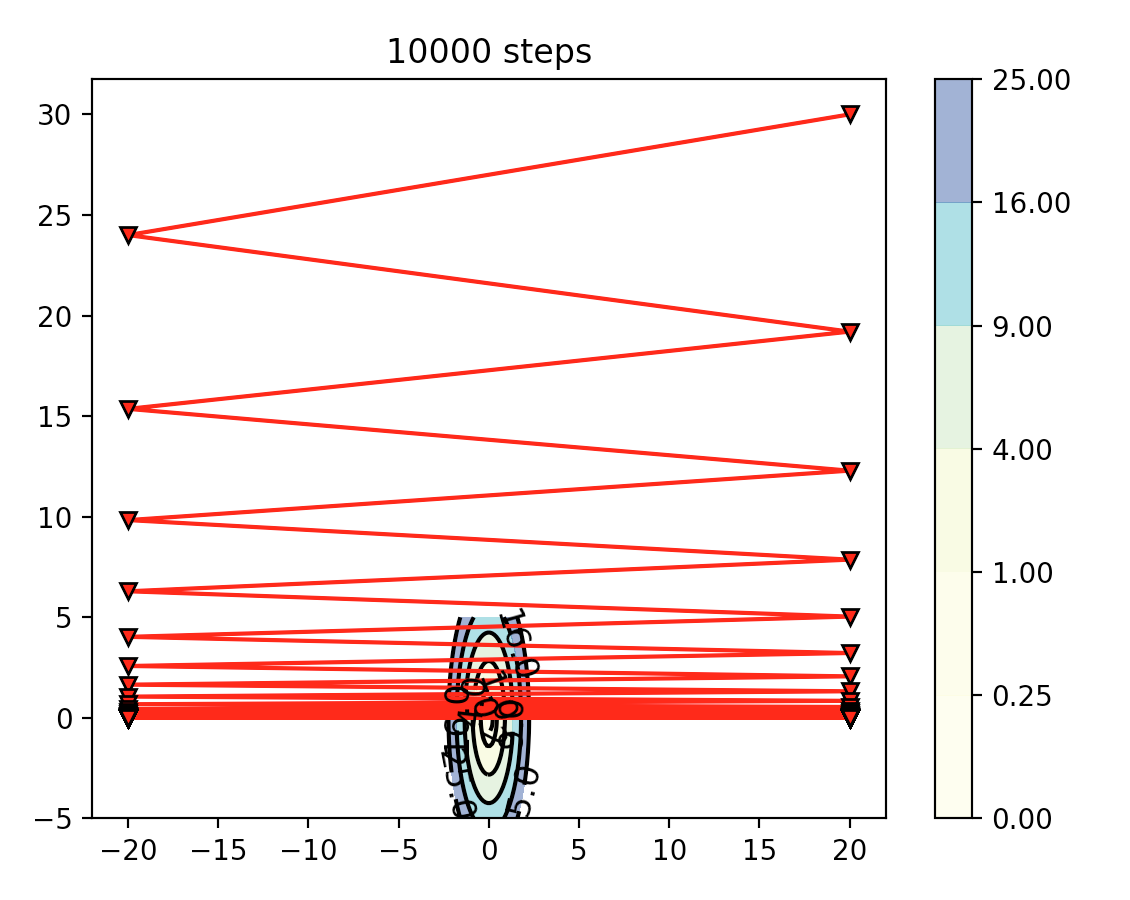
\includegraphics[width=0.49\linewidth]{18.png} \\
 a)$M,\ x_1$ & b)$M,\ x_2$\\
\end{tabular}
\end{center}

$\bullet$ Armijo

Видно что метод очень чувствутелен к обусловленности функции. Так же есть небольшая зависимость о выбора начальной точки.

\begin{center}
\begin{tabular}{cc}
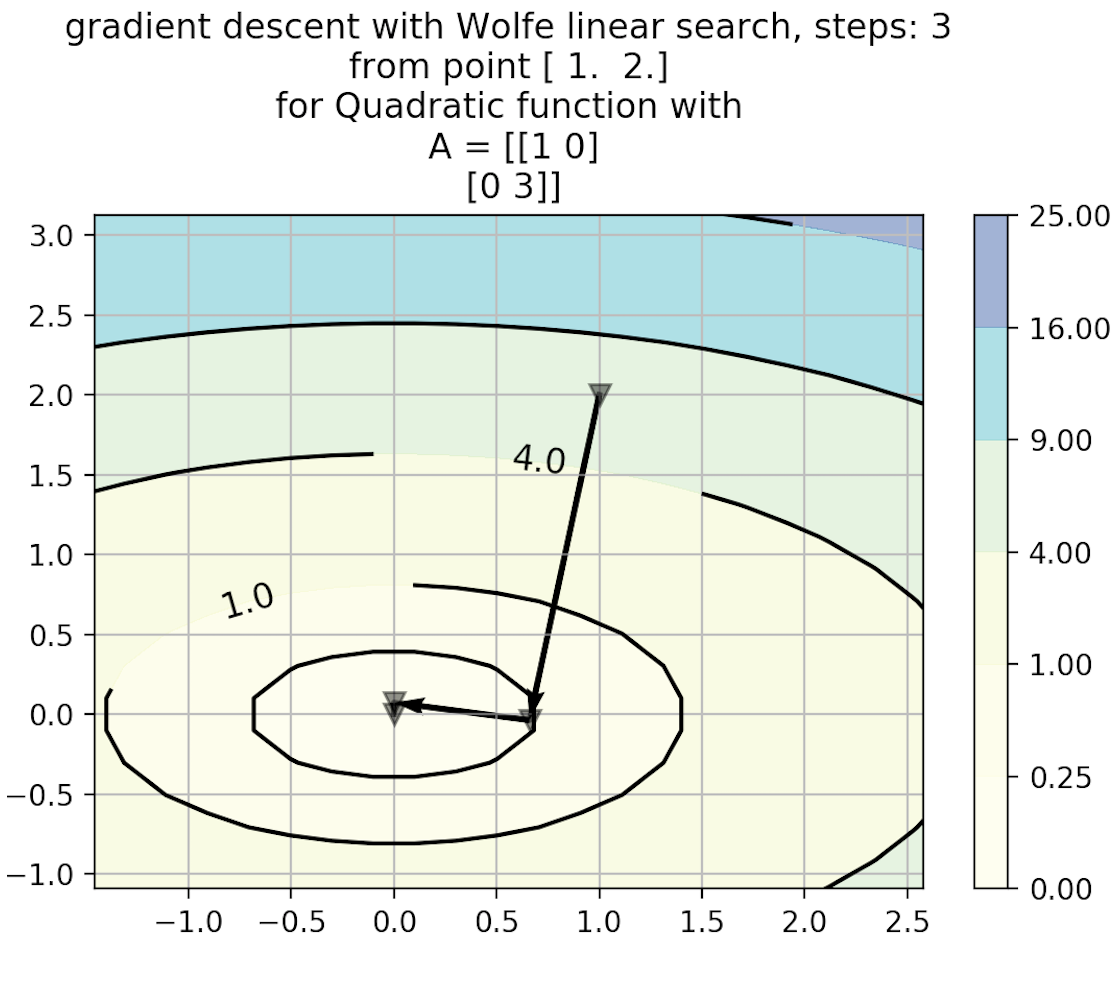
\includegraphics[width=0.49\linewidth]{11.png} &
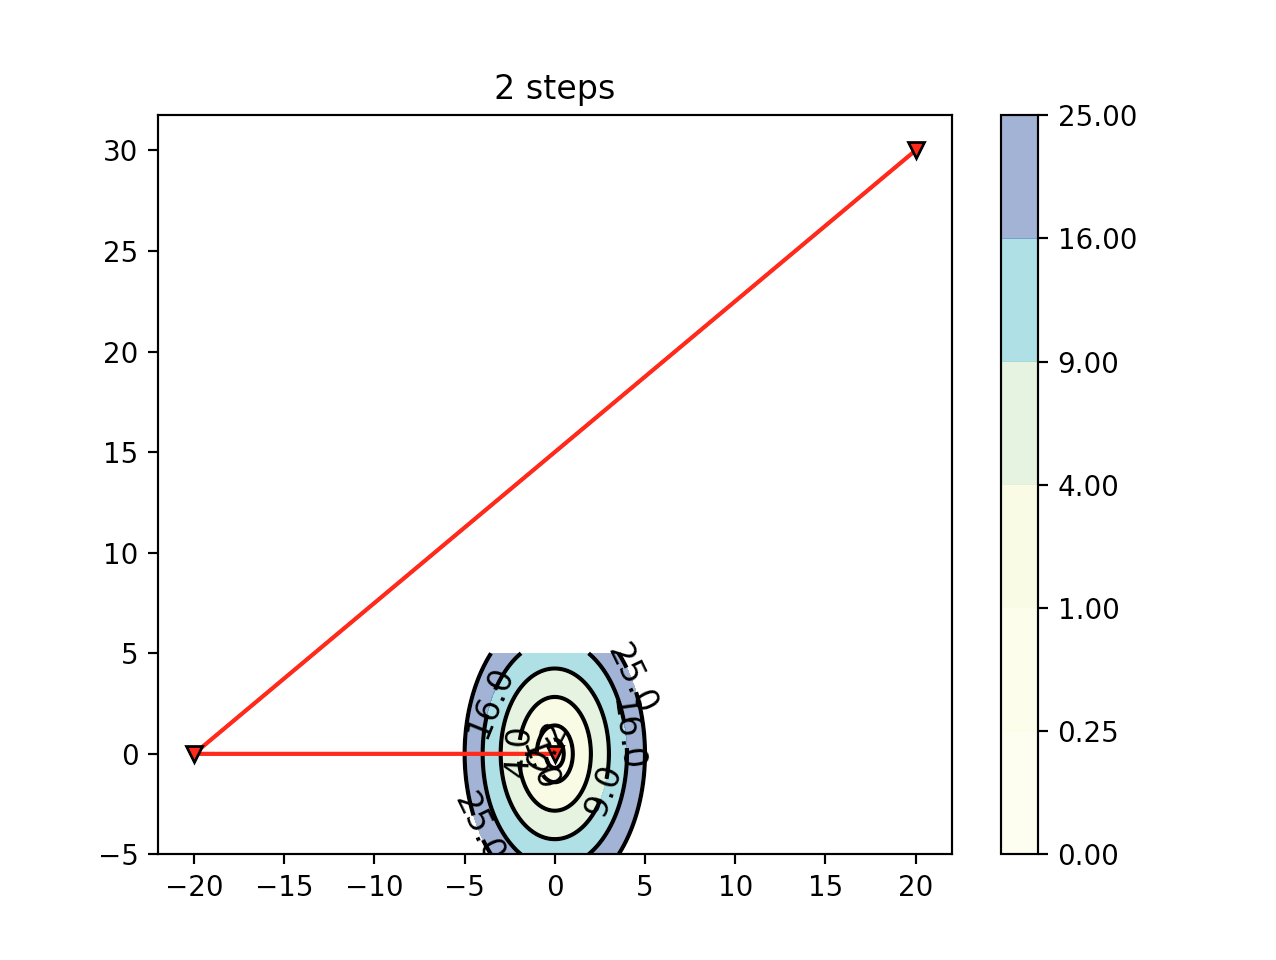
\includegraphics[width=0.49\linewidth]{12.png} \\
 a)$M_1,\ x_1$ & b)$M_1,\ x_2$\\
\end{tabular}
\end{center}

\begin{center}
\begin{tabular}{cc}
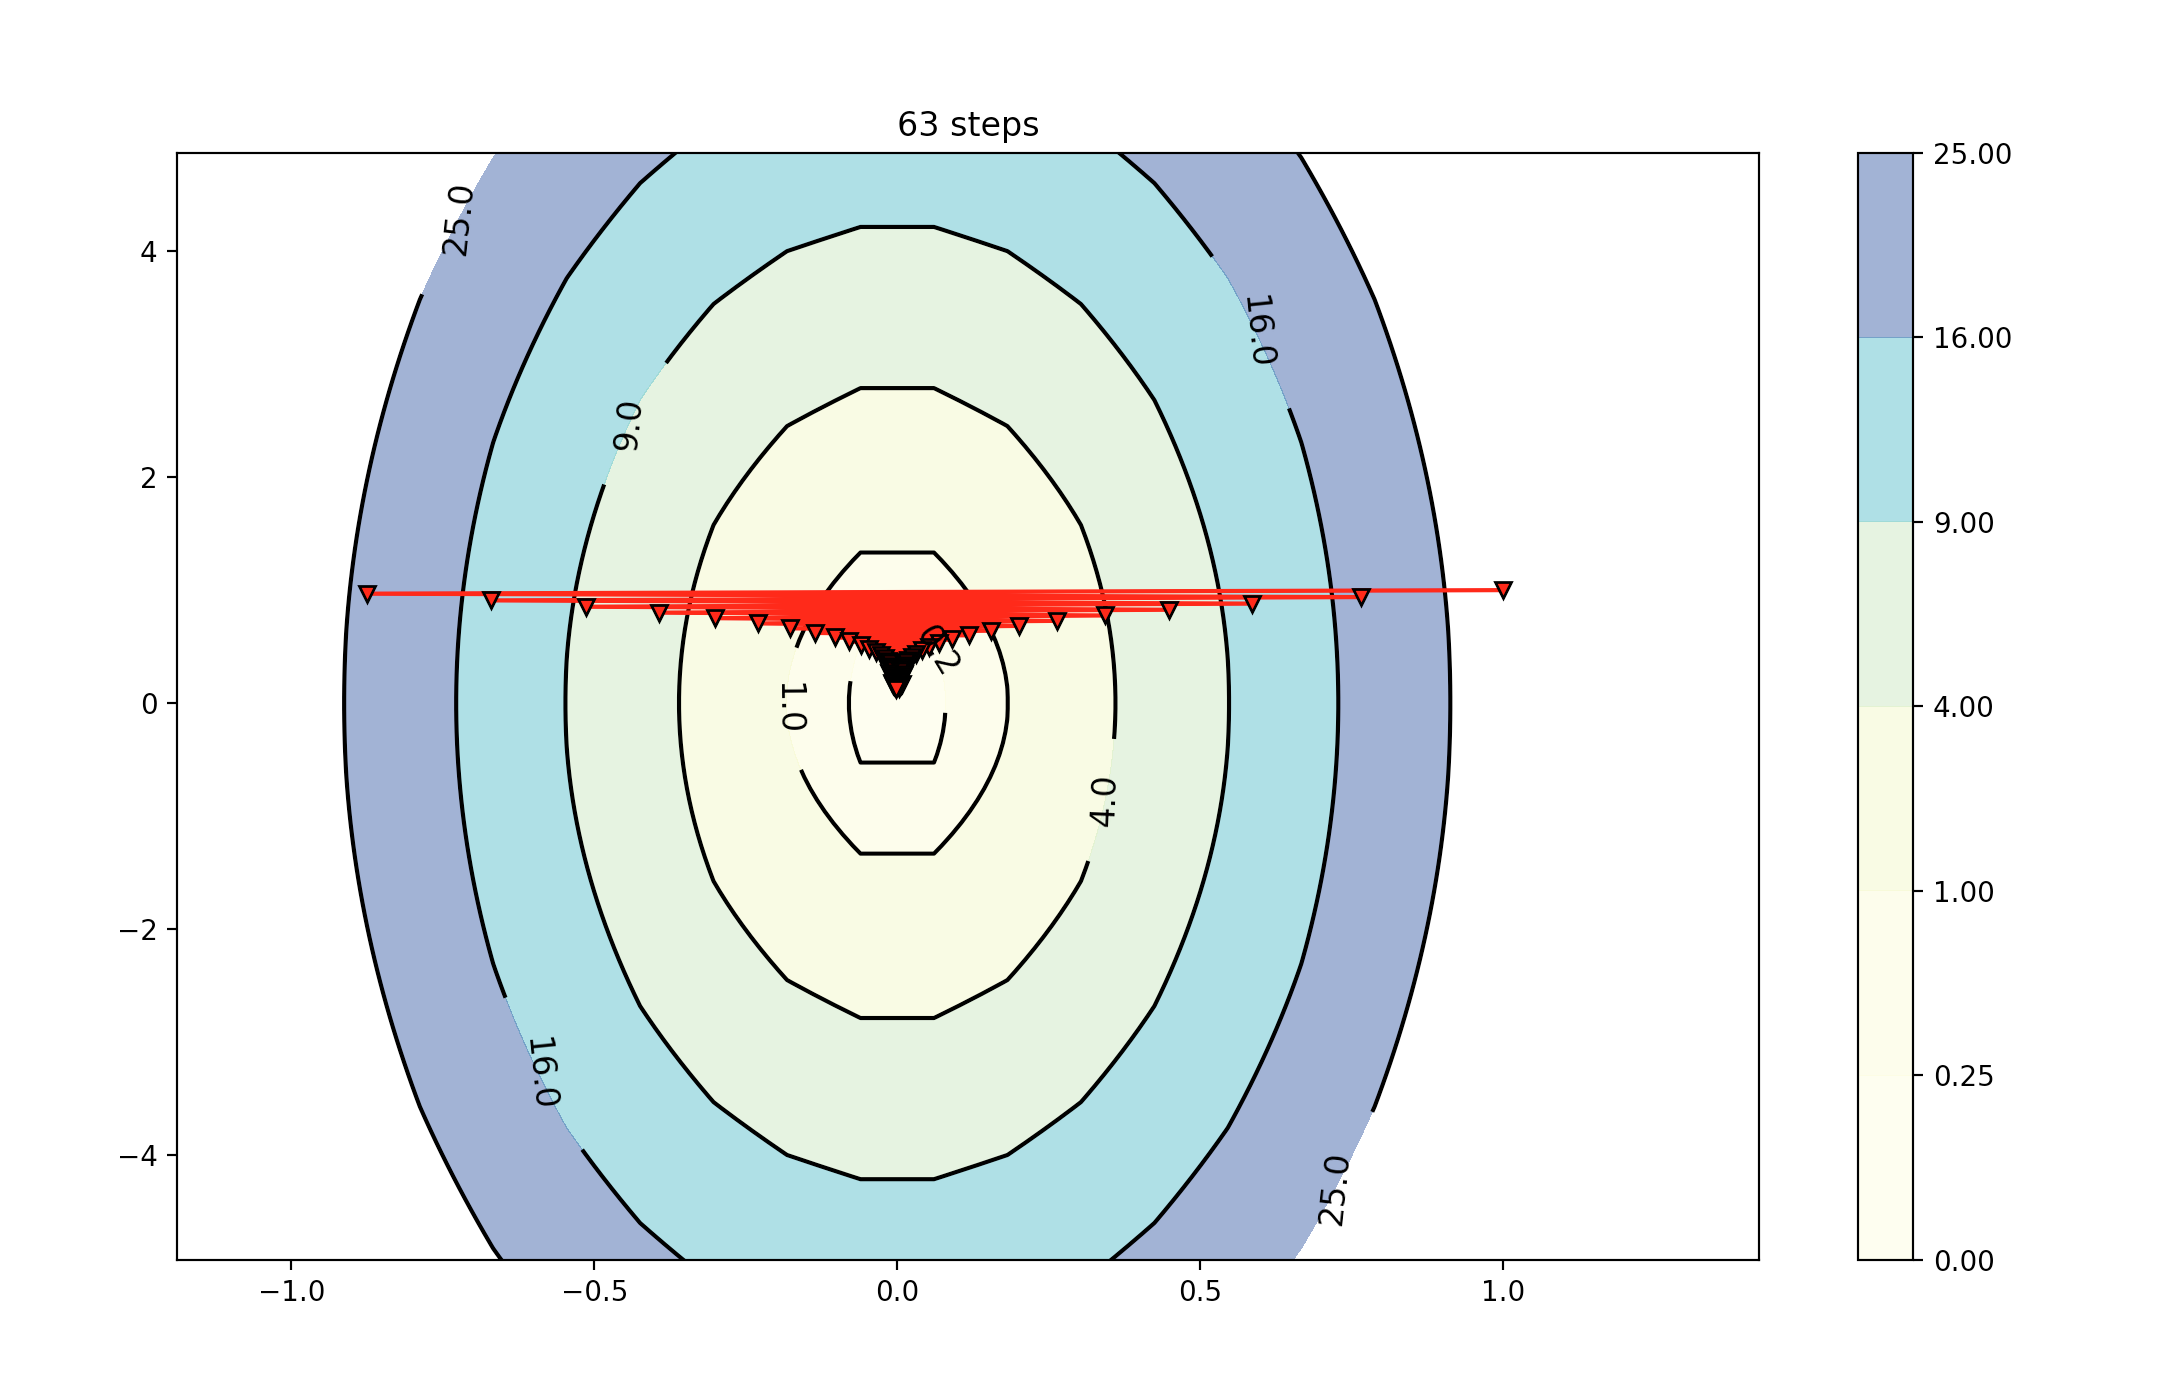
\includegraphics[width=0.49\linewidth]{13.png} &
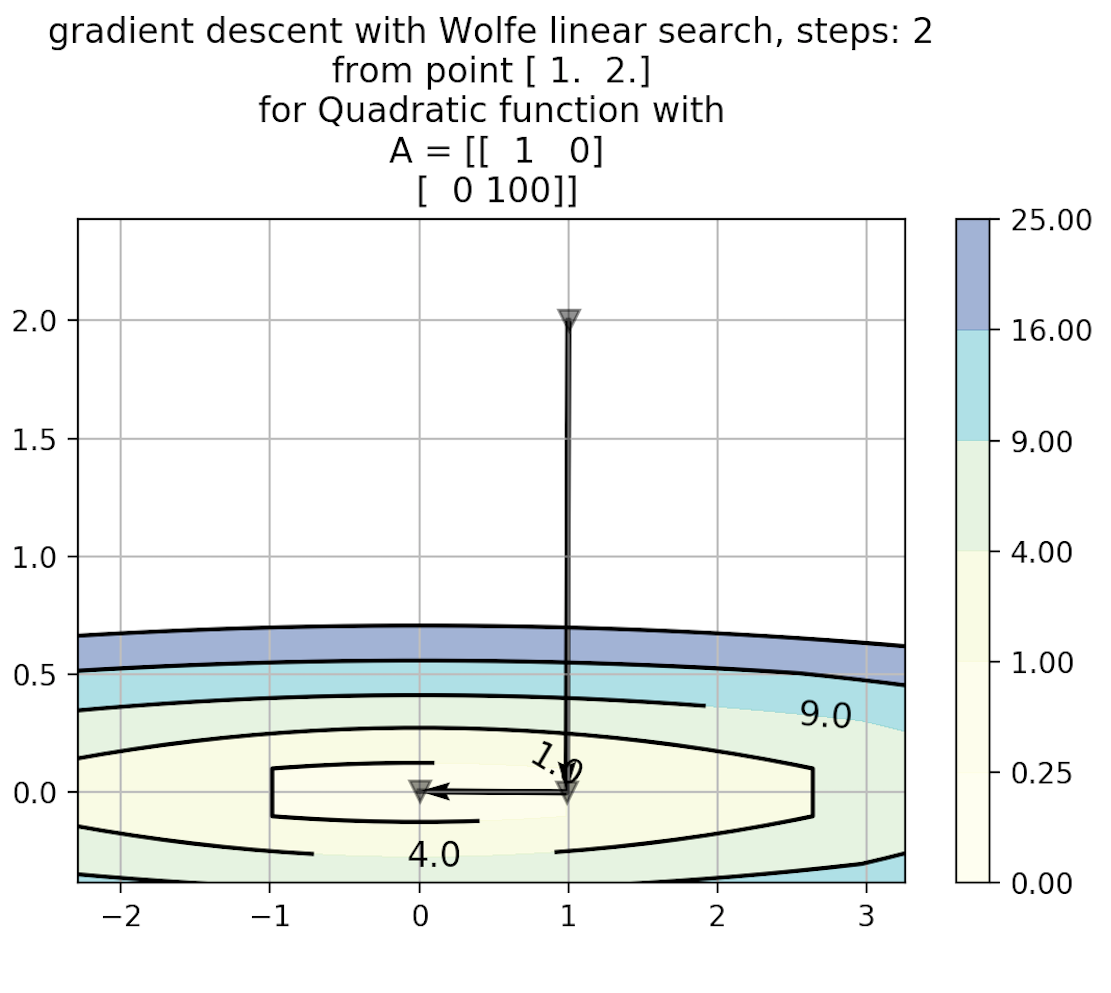
\includegraphics[width=0.49\linewidth]{14.png} \\
 a)$M_2,\ x_1$ & b)$M_2,\ x_2$\\
\end{tabular}
\end{center}


Зависимость поведения метода от начальной точки

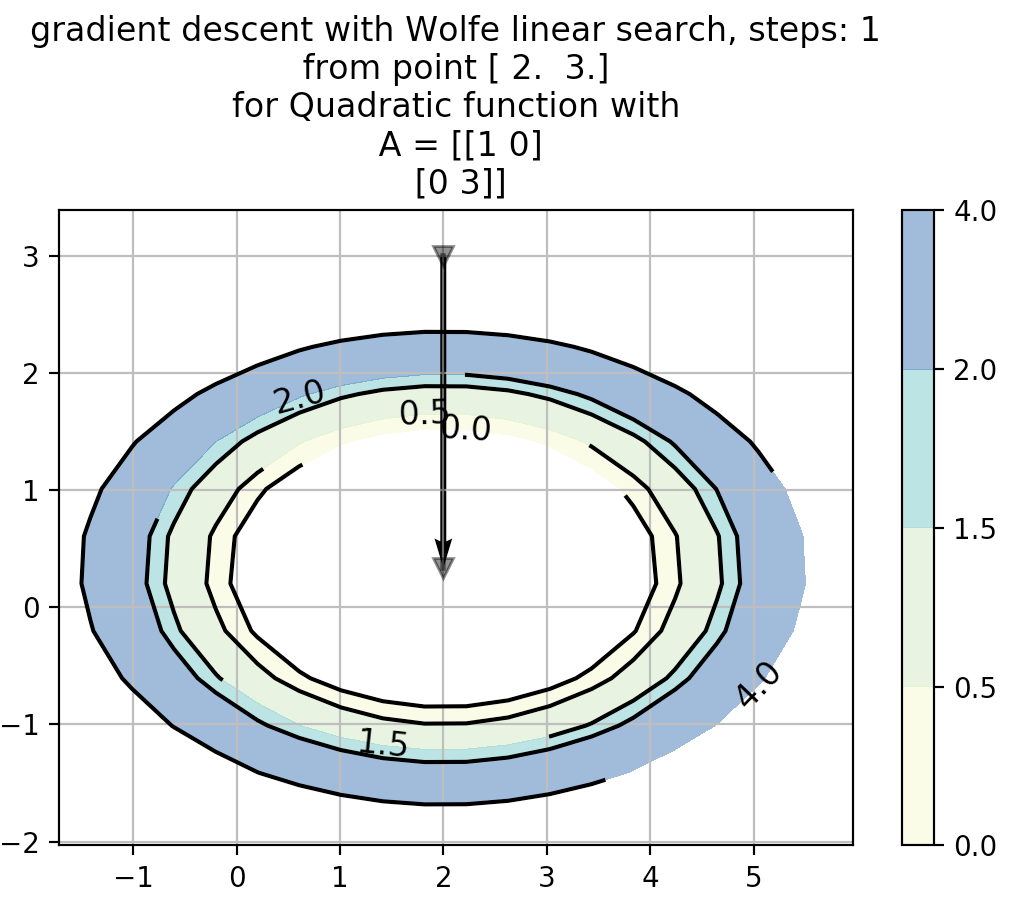
\includegraphics[width=0.5 \textwidth]{121.png}
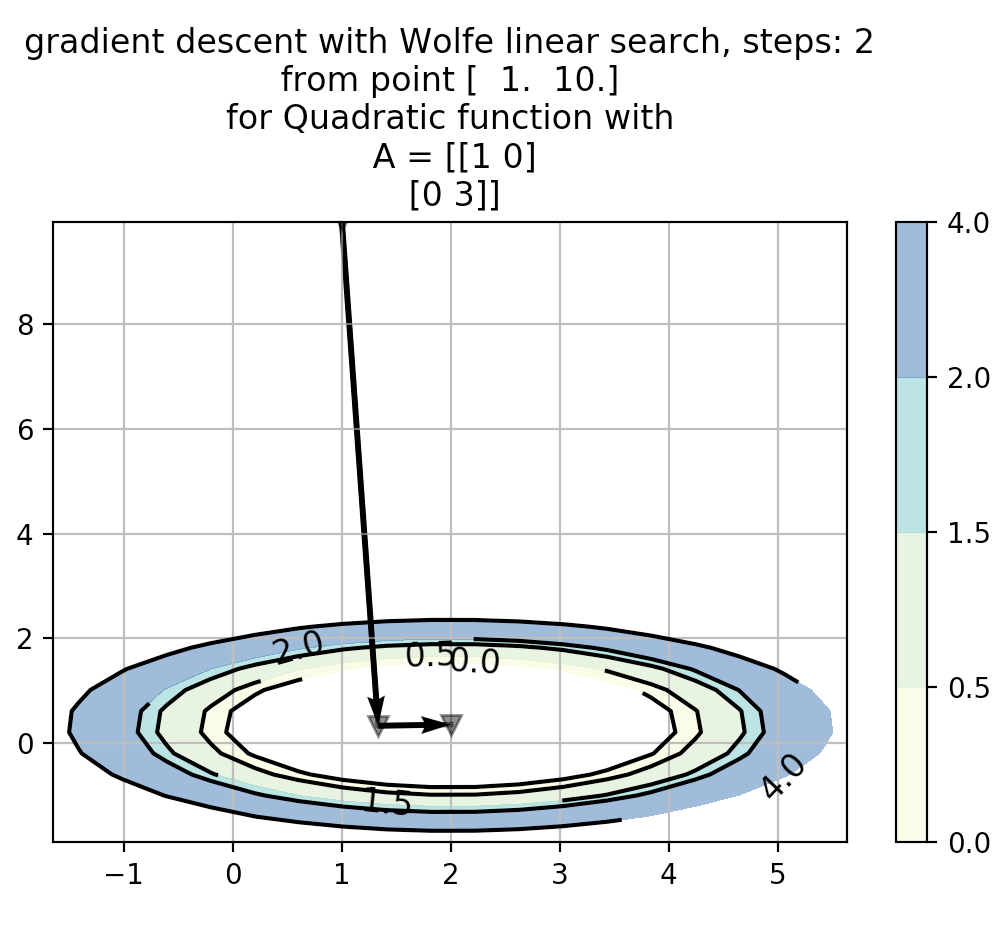
\includegraphics[width=0.5 \textwidth]{122.png}

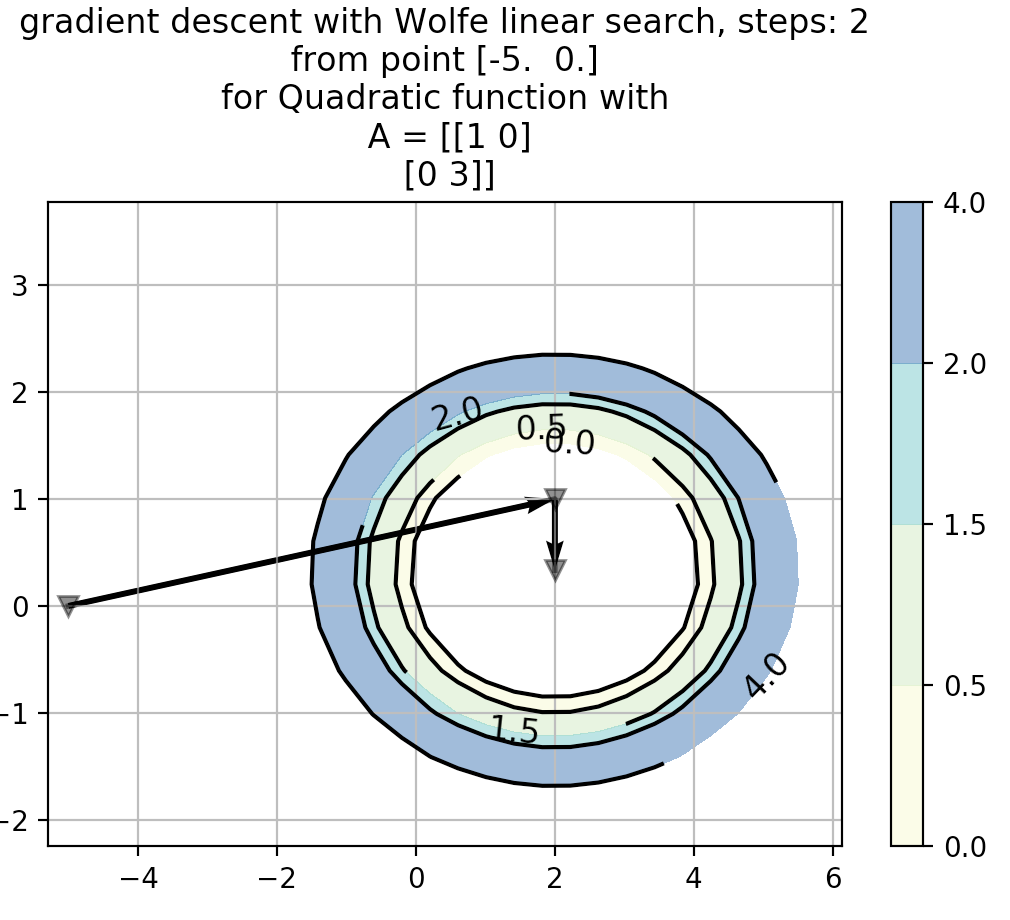
\includegraphics[width=0.5 \textwidth]{123.png}
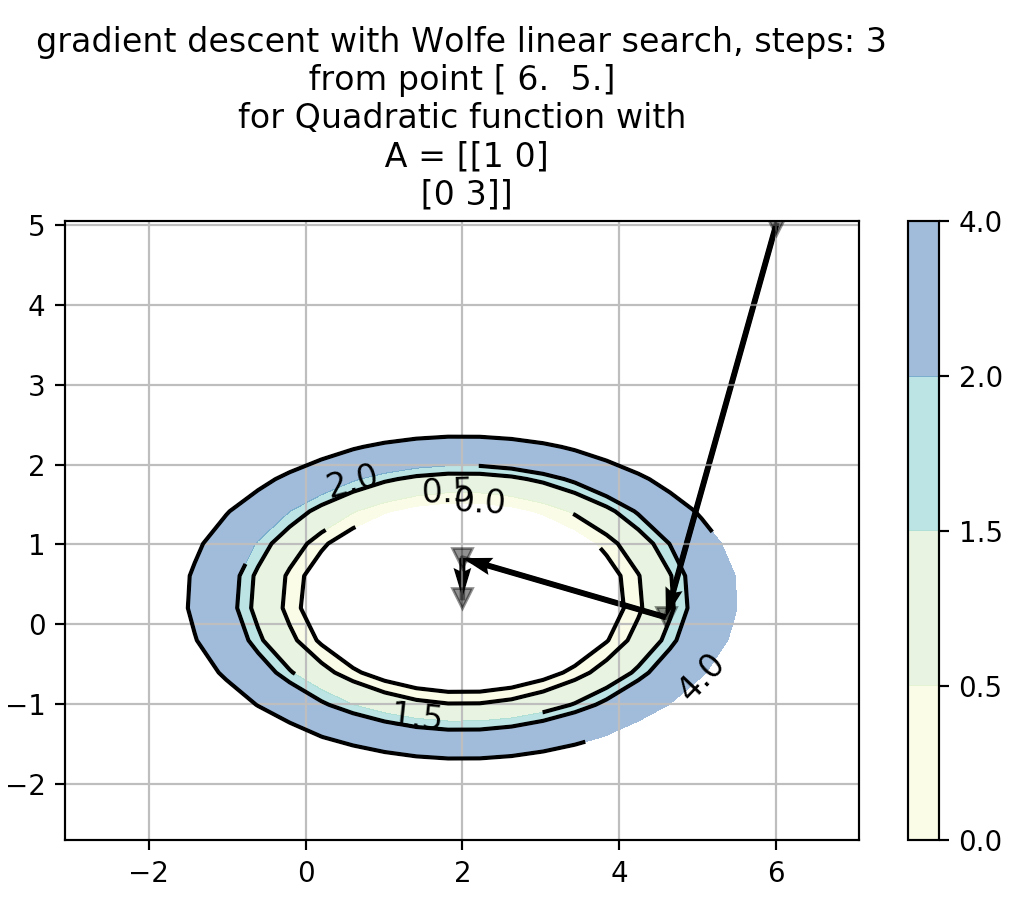
\includegraphics[width=0.5 \textwidth]{124.png}

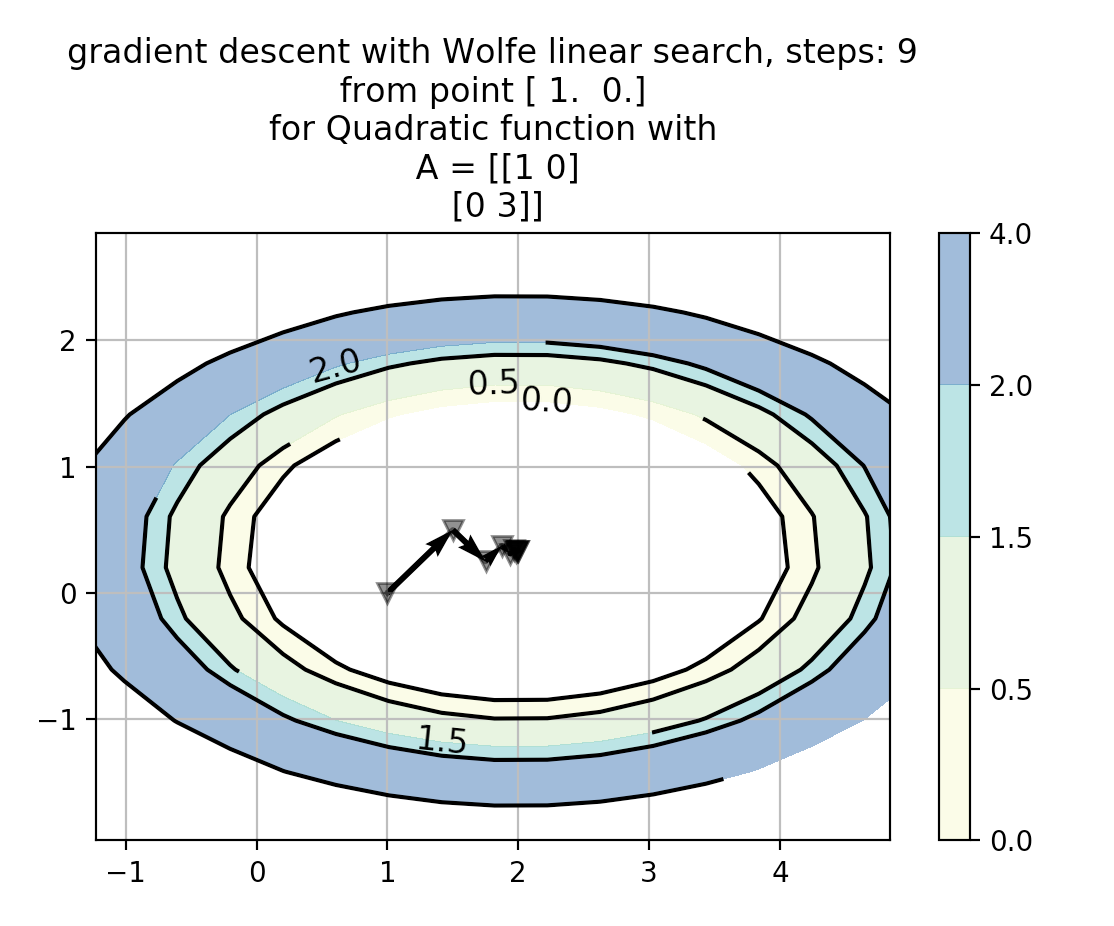
\includegraphics[width=0.5 \textwidth]{125.png}


Зависимость поведения метода от стратегии выбора шага.

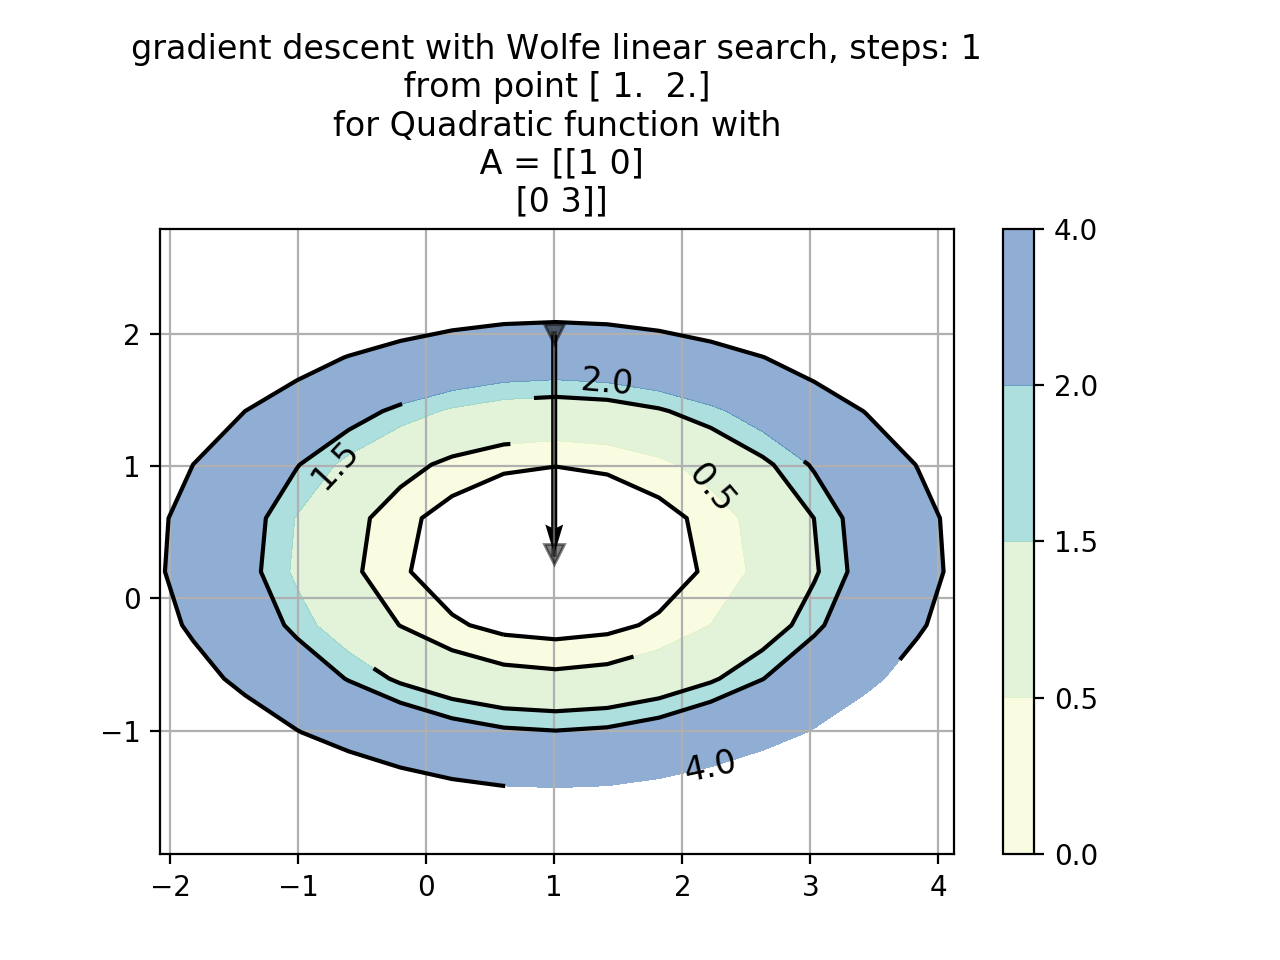
\includegraphics[width=0.6 \textwidth]{131.png}
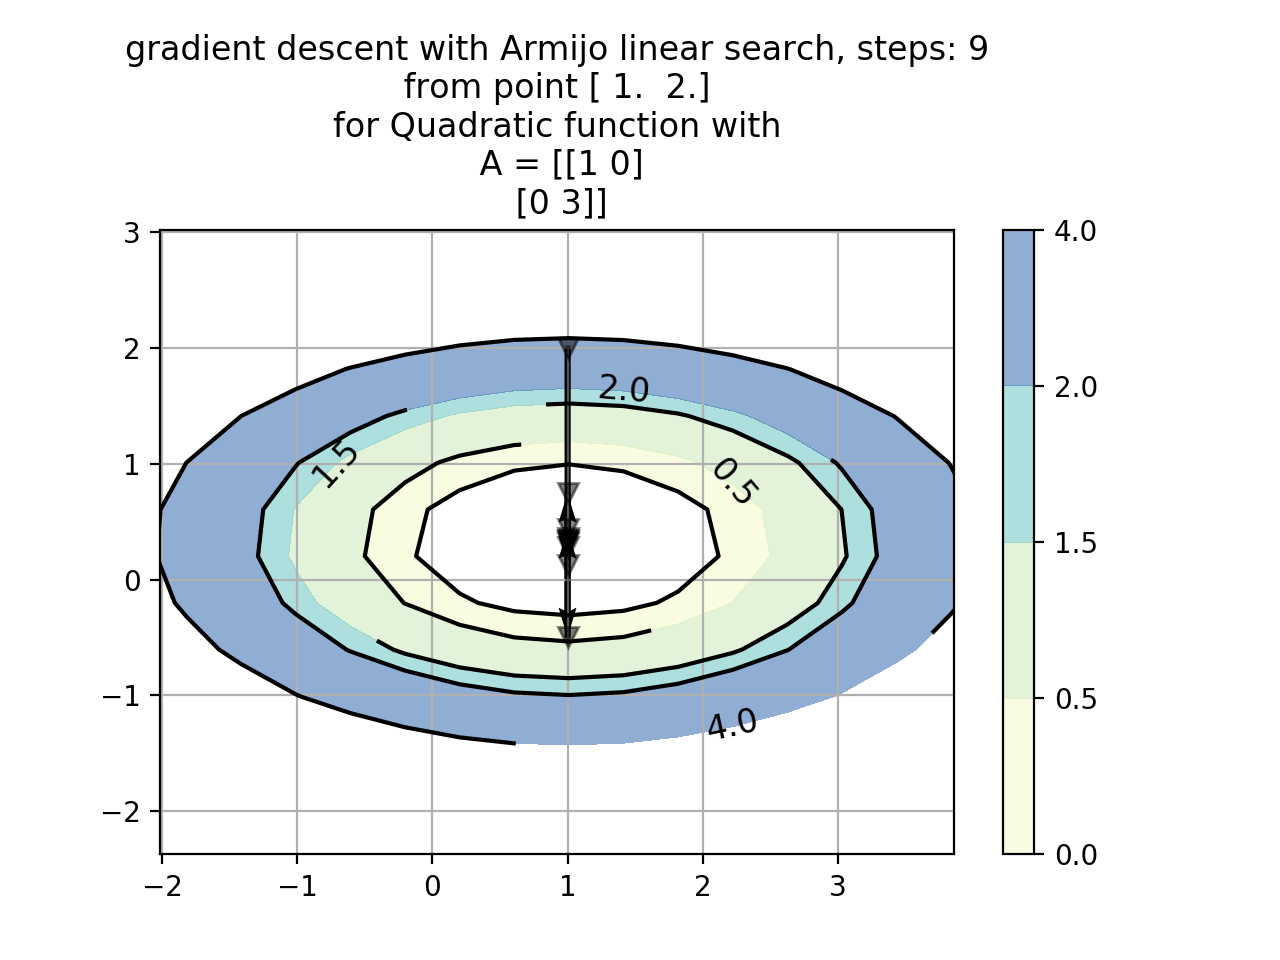
\includegraphics[width=0.6 \textwidth]{132.png}

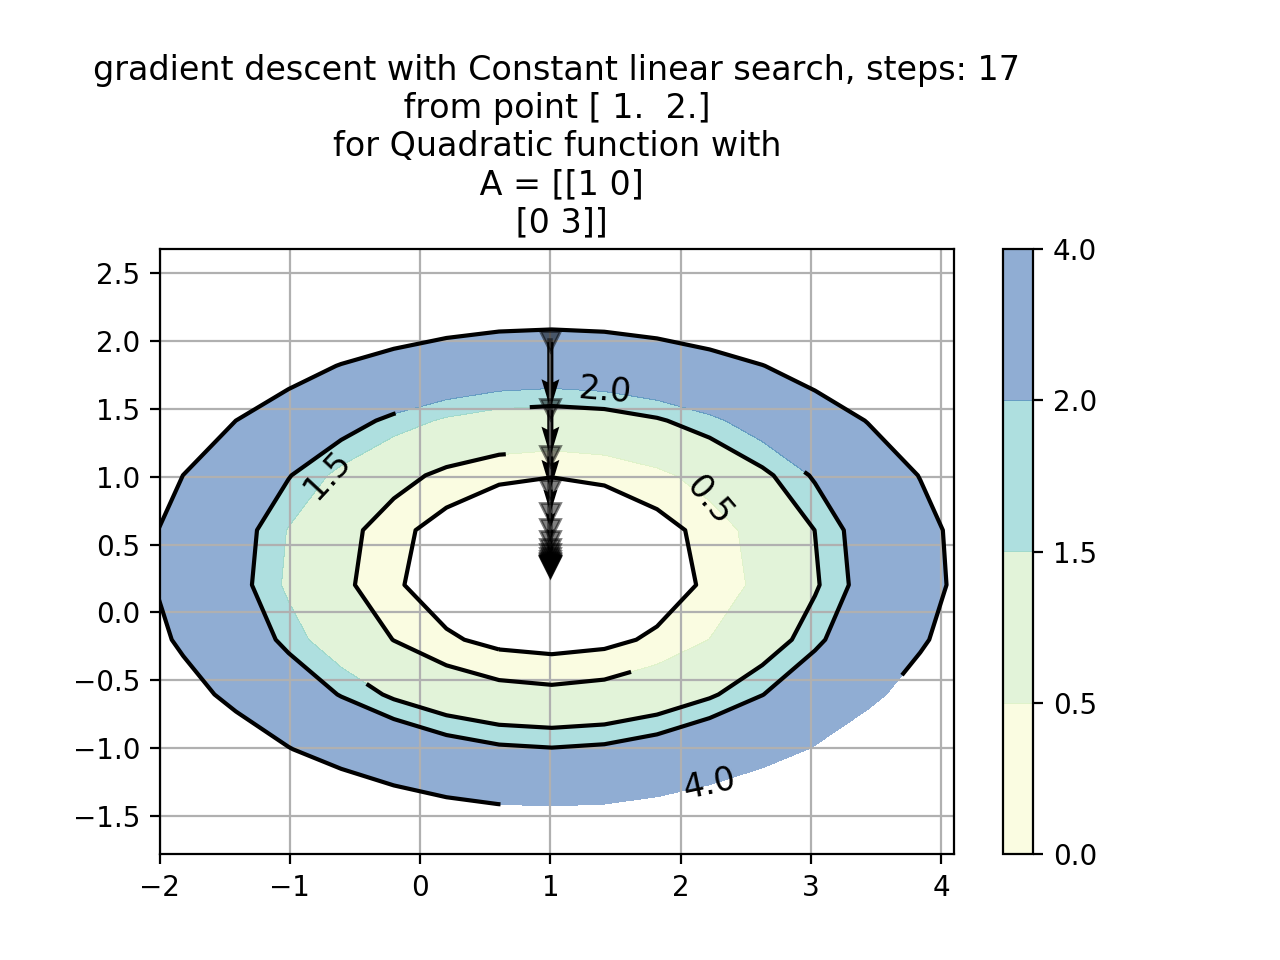
\includegraphics[width=0.6 \textwidth]{133.png}

Зависимость числа итераций градиентного спуска от числа обусловленности и размерности пространства.

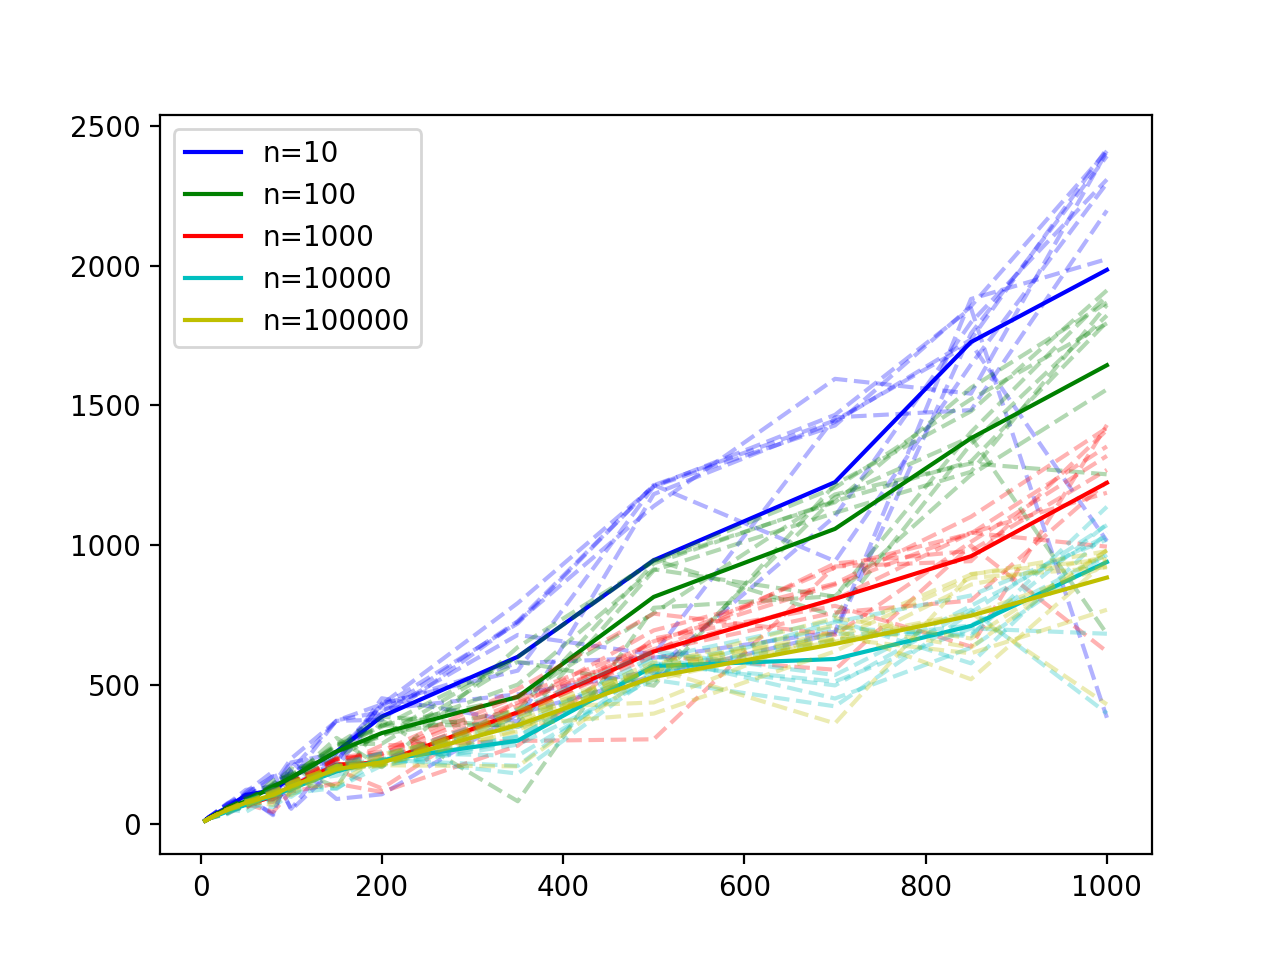
\includegraphics[width=1 \textwidth]{21.png}

Сравнение методов градиентного спуска и Ньютона на реальной задаче логистической регрессии.

w8a

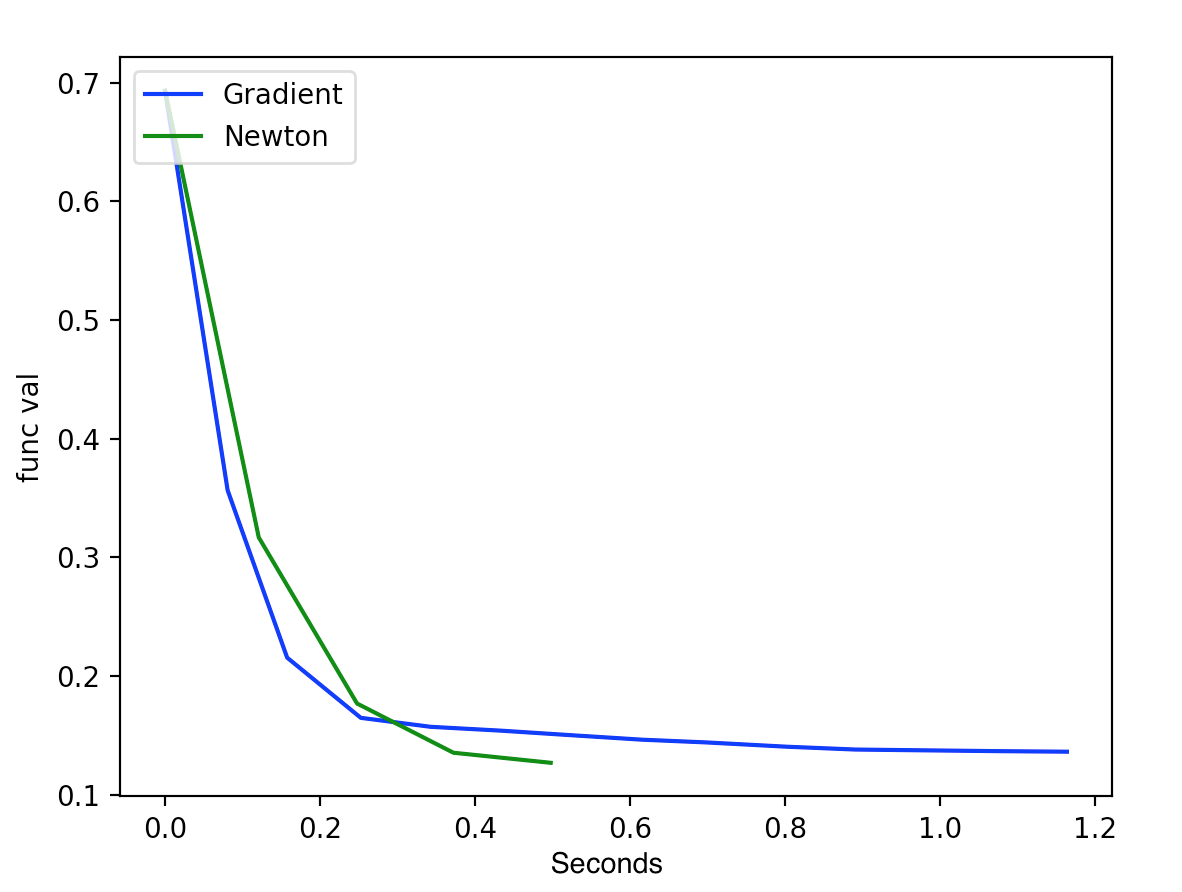
\includegraphics[width=0.6 \textwidth]{31.png}
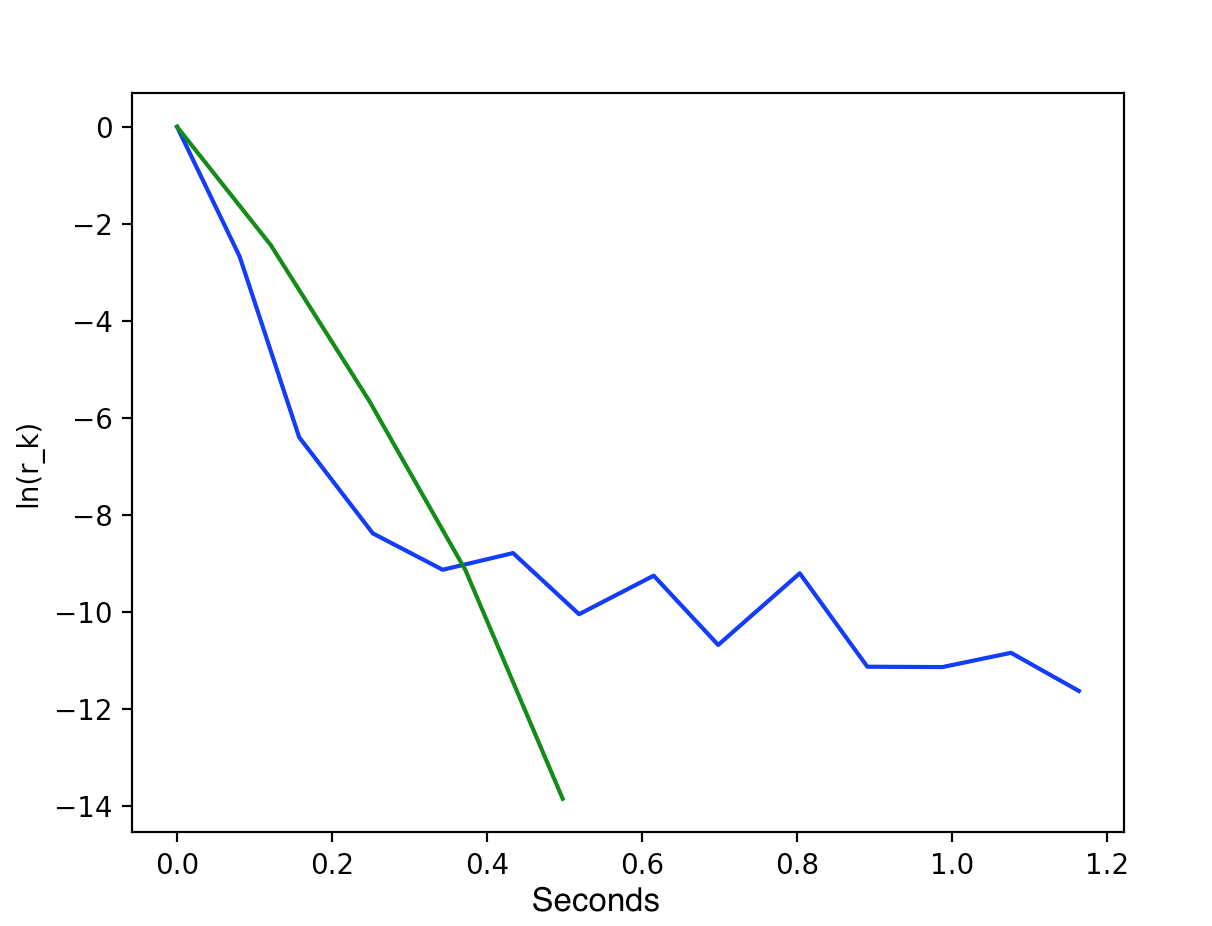
\includegraphics[width=0.6 \textwidth]{32.png}

gisette-scale

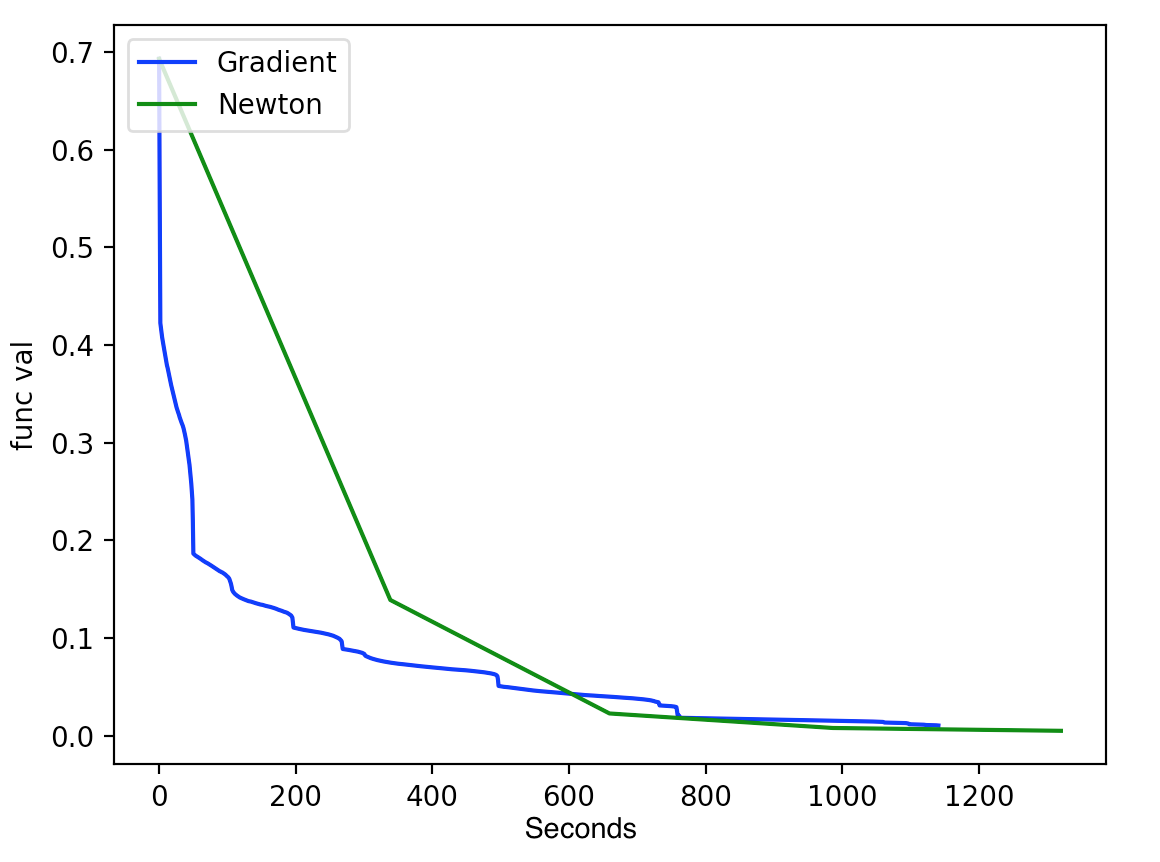
\includegraphics[width=0.6 \textwidth]{33.png}
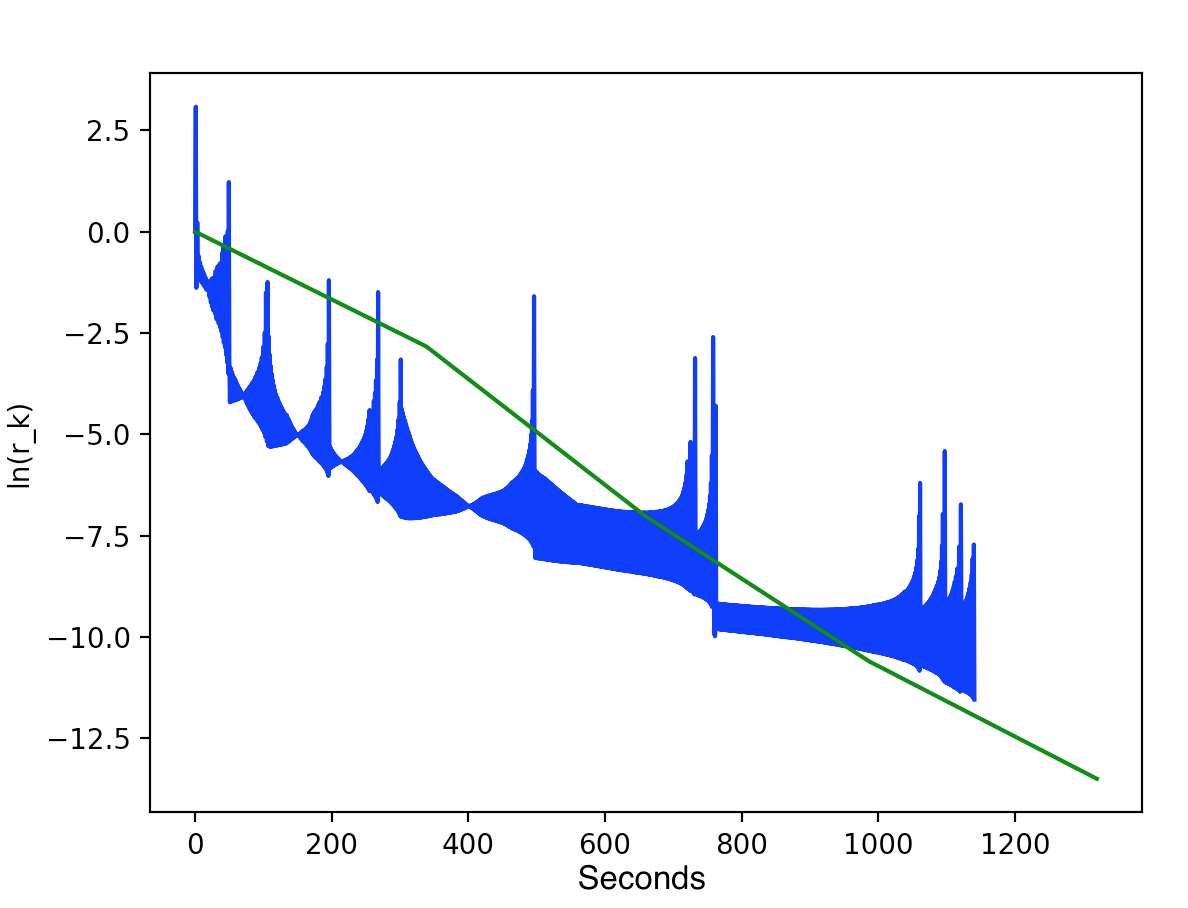
\includegraphics[width=0.6 \textwidth]{34.png}

real-sim

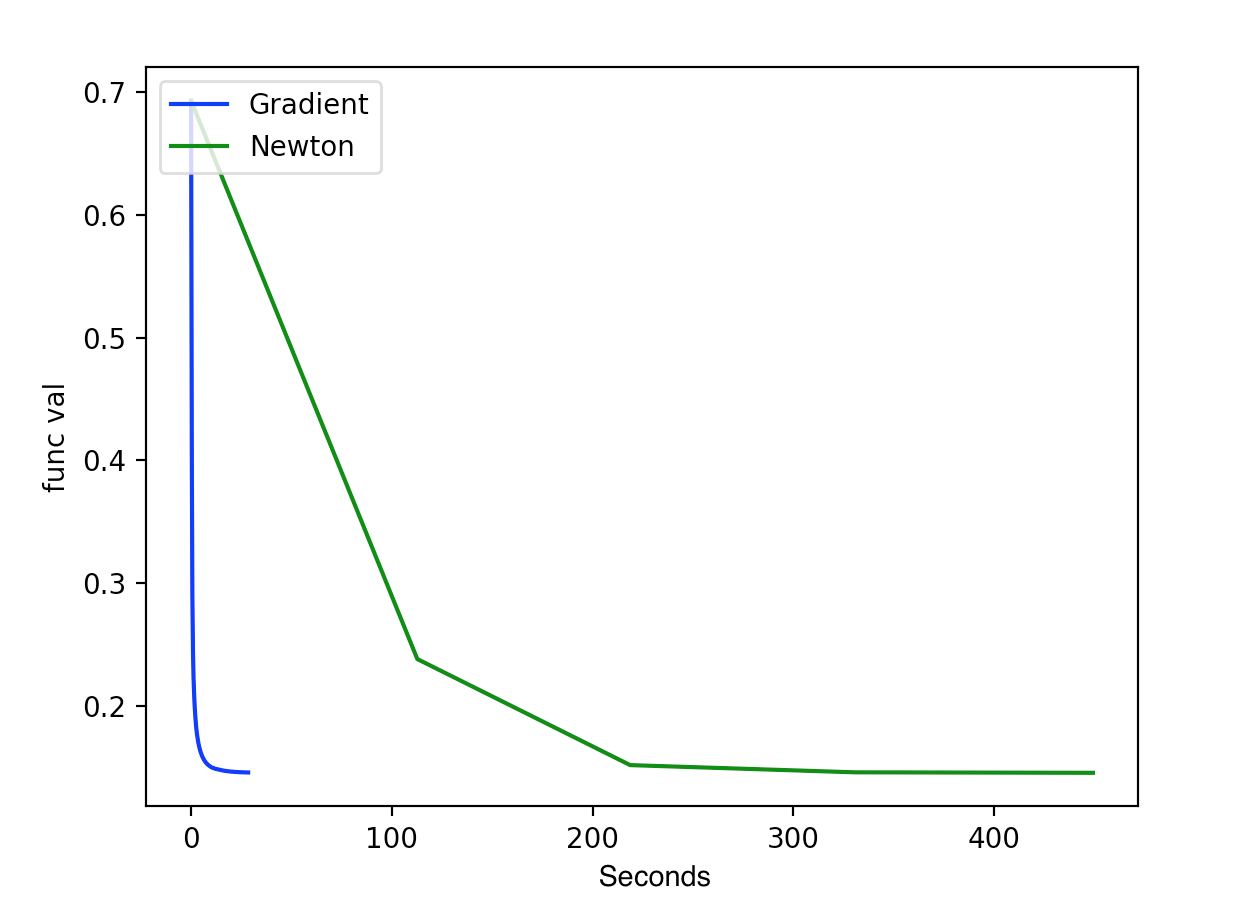
\includegraphics[width=0.6 \textwidth]{35.png}
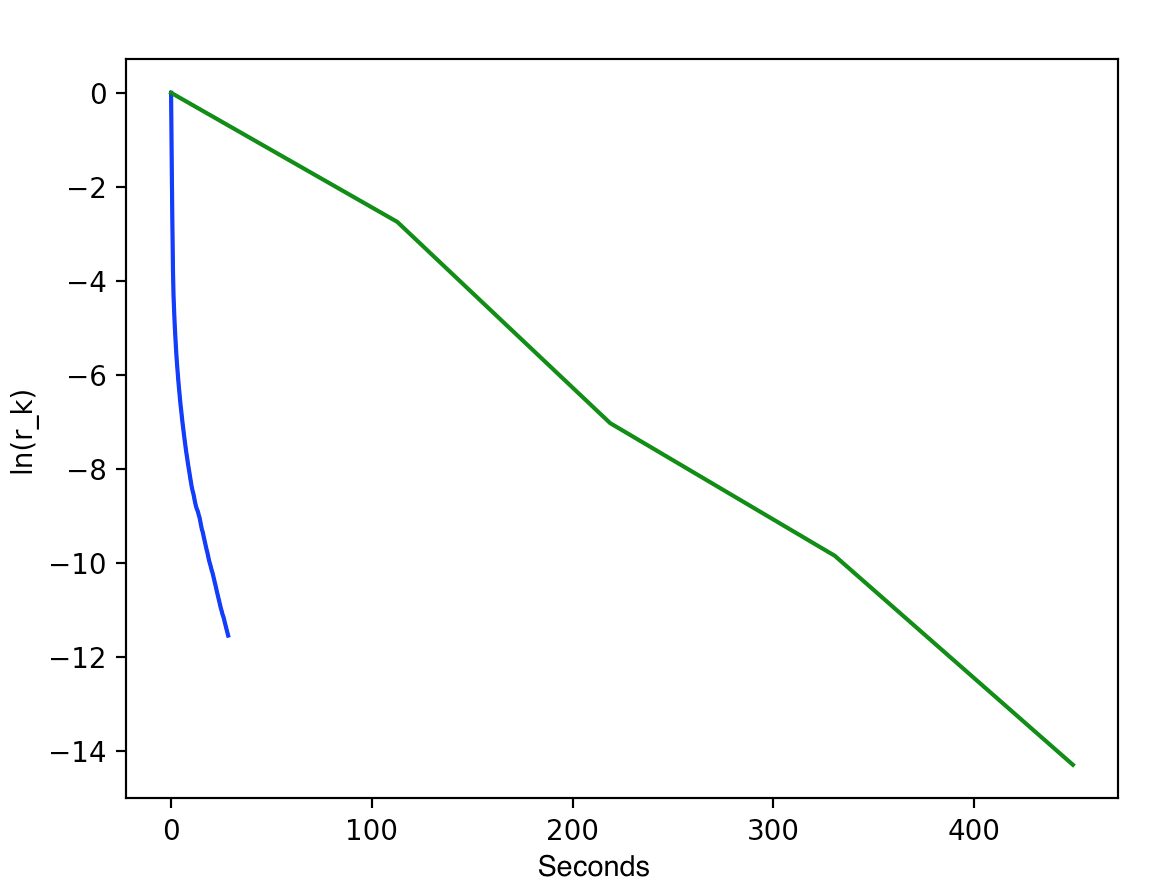
\includegraphics[width=0.6 \textwidth]{36.png}

Оптимизация вычислений в градиентном спуске.


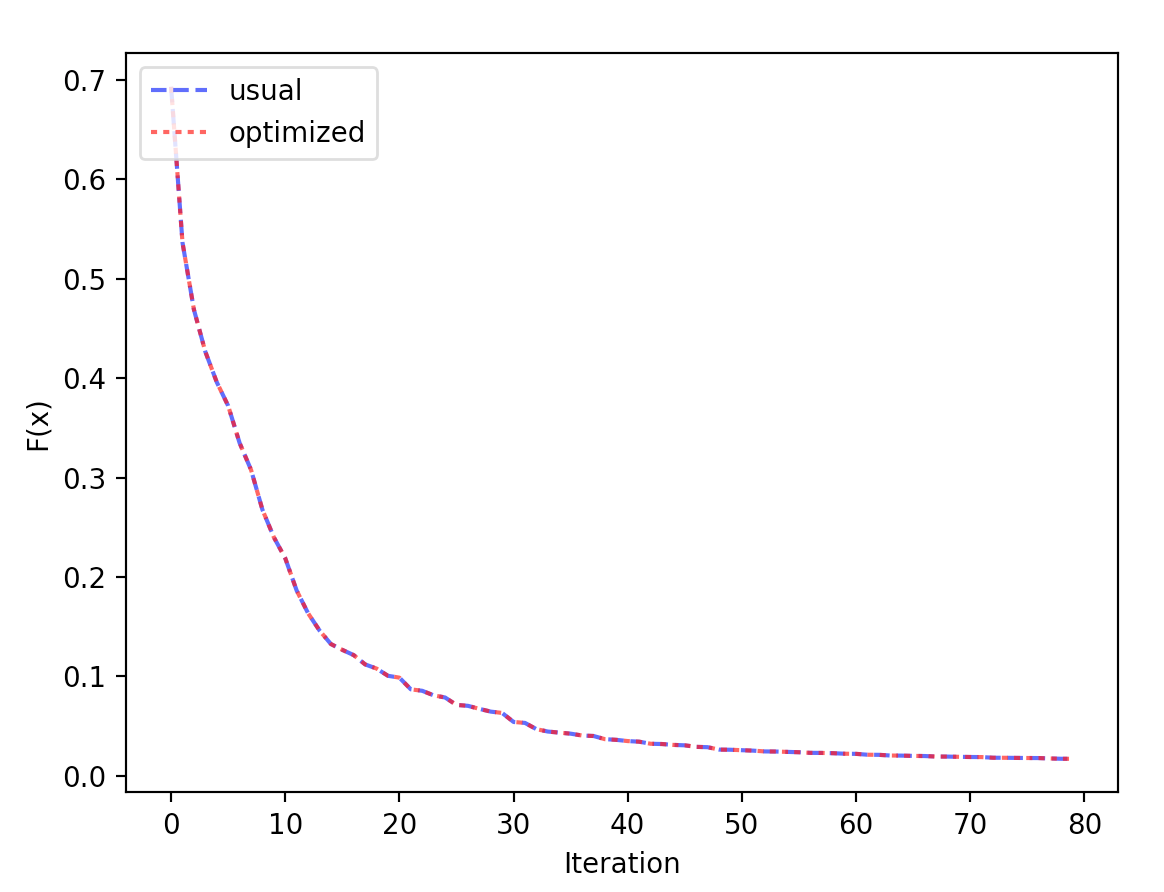
\includegraphics[width=0.6 \textwidth]{41.png}


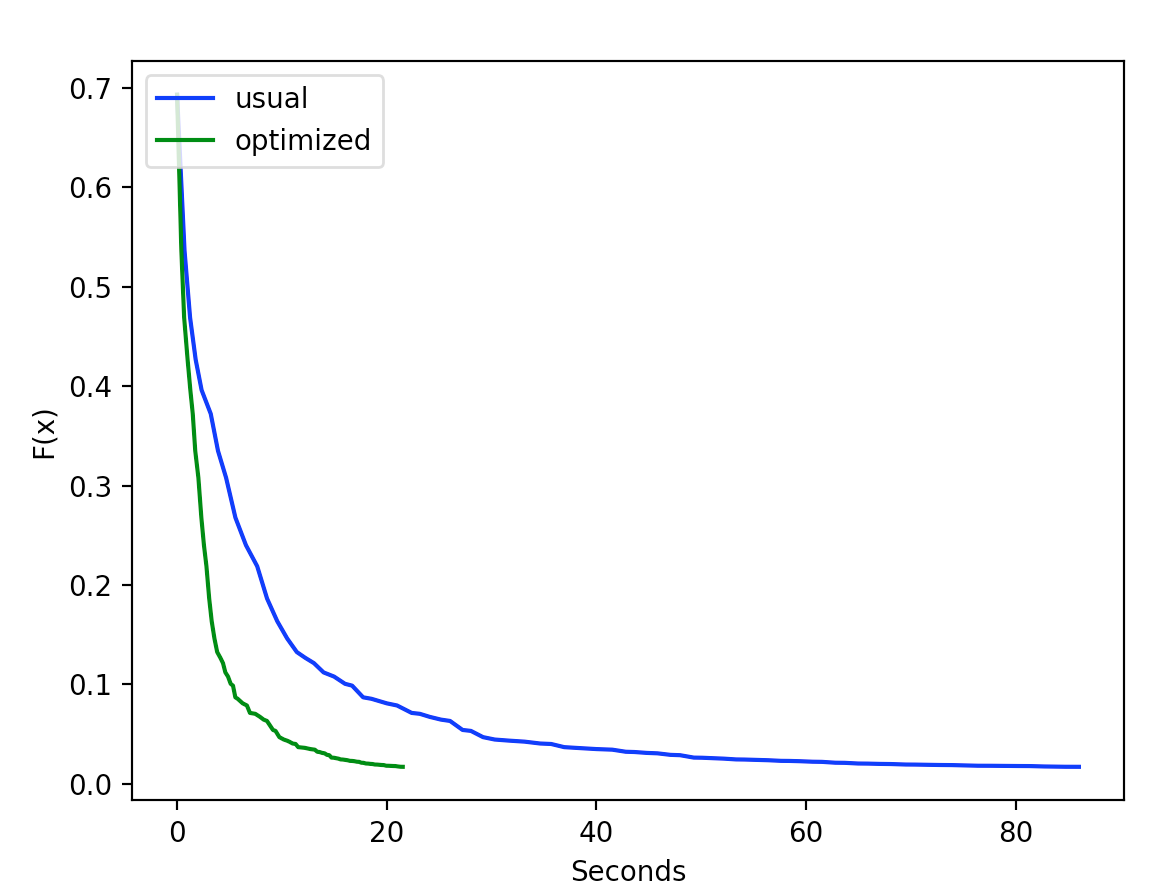
\includegraphics[width=0.6 \textwidth]{42.png}
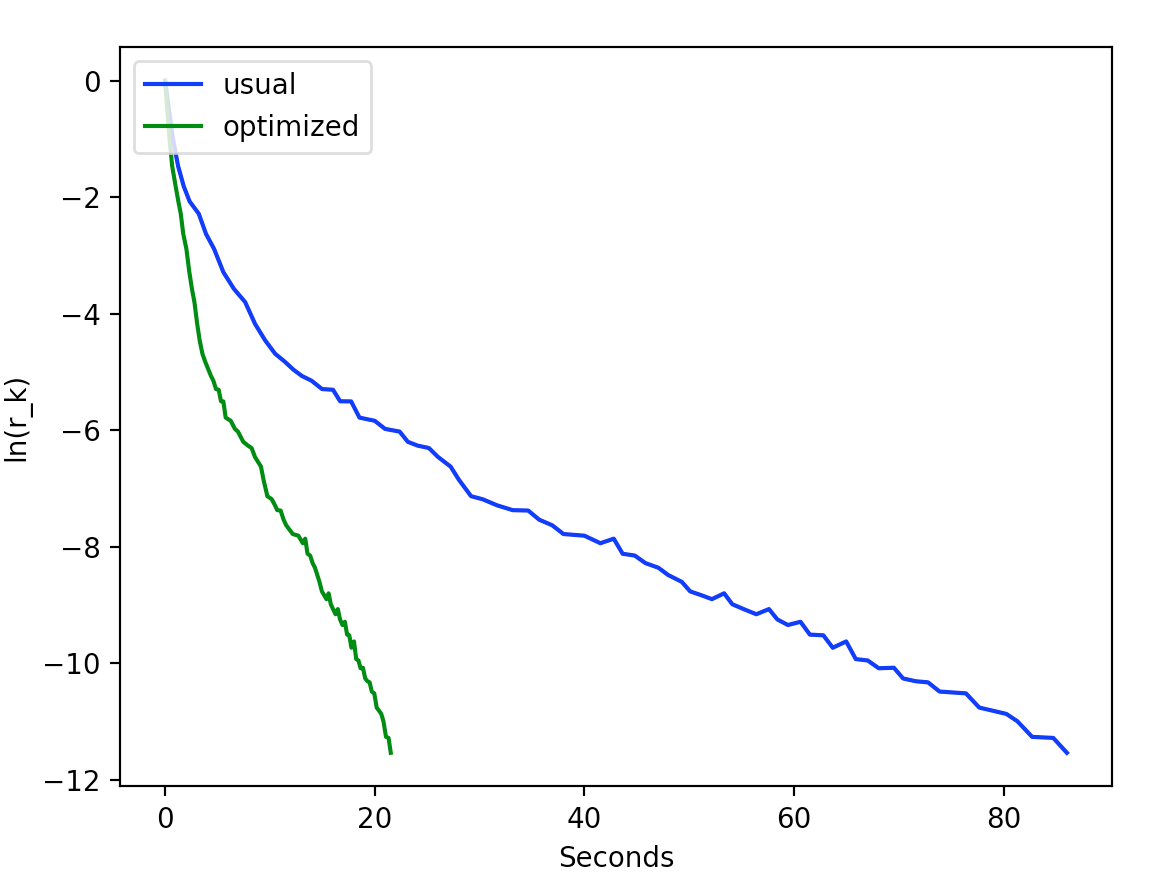
\includegraphics[width=0.6 \textwidth]{43.png}



Стратегия выбора длины шага в градиентном спуске

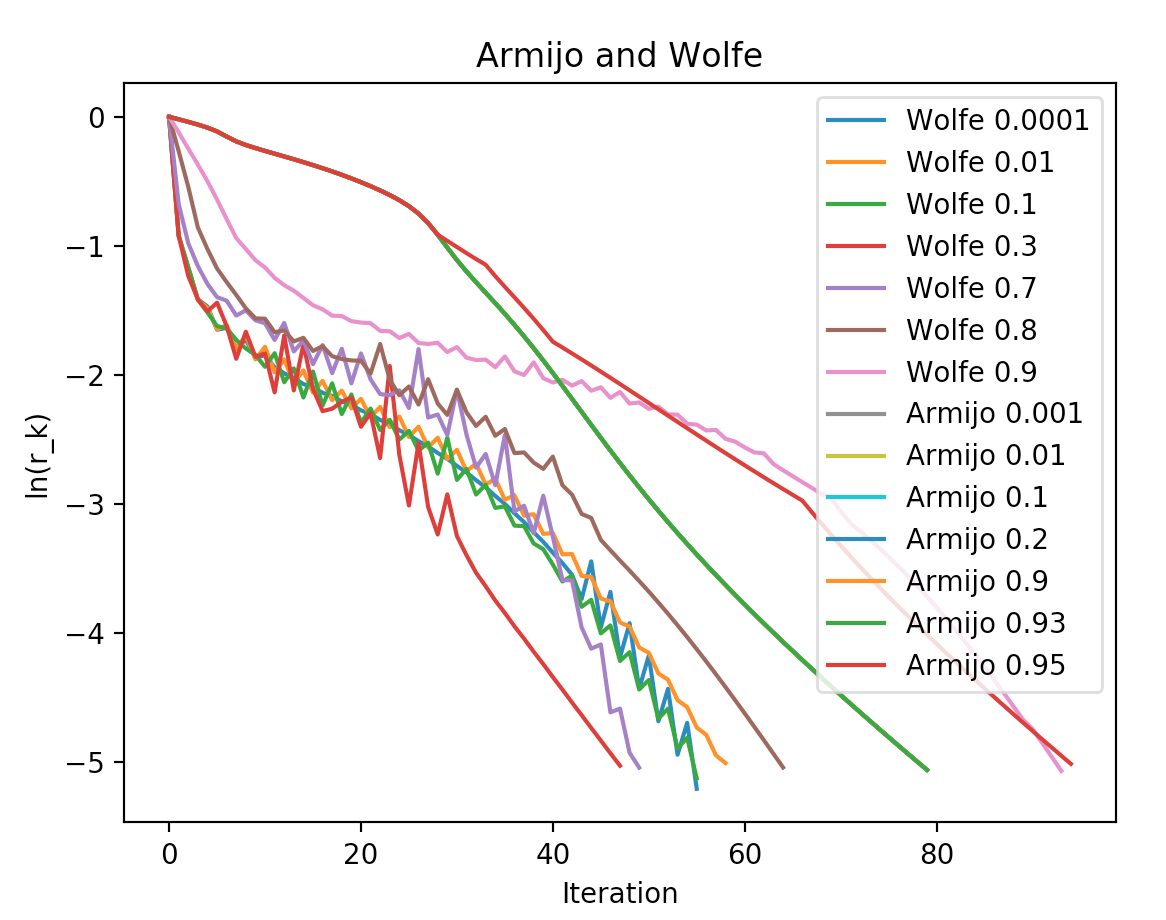
\includegraphics[width=0.6 \textwidth]{51.png}
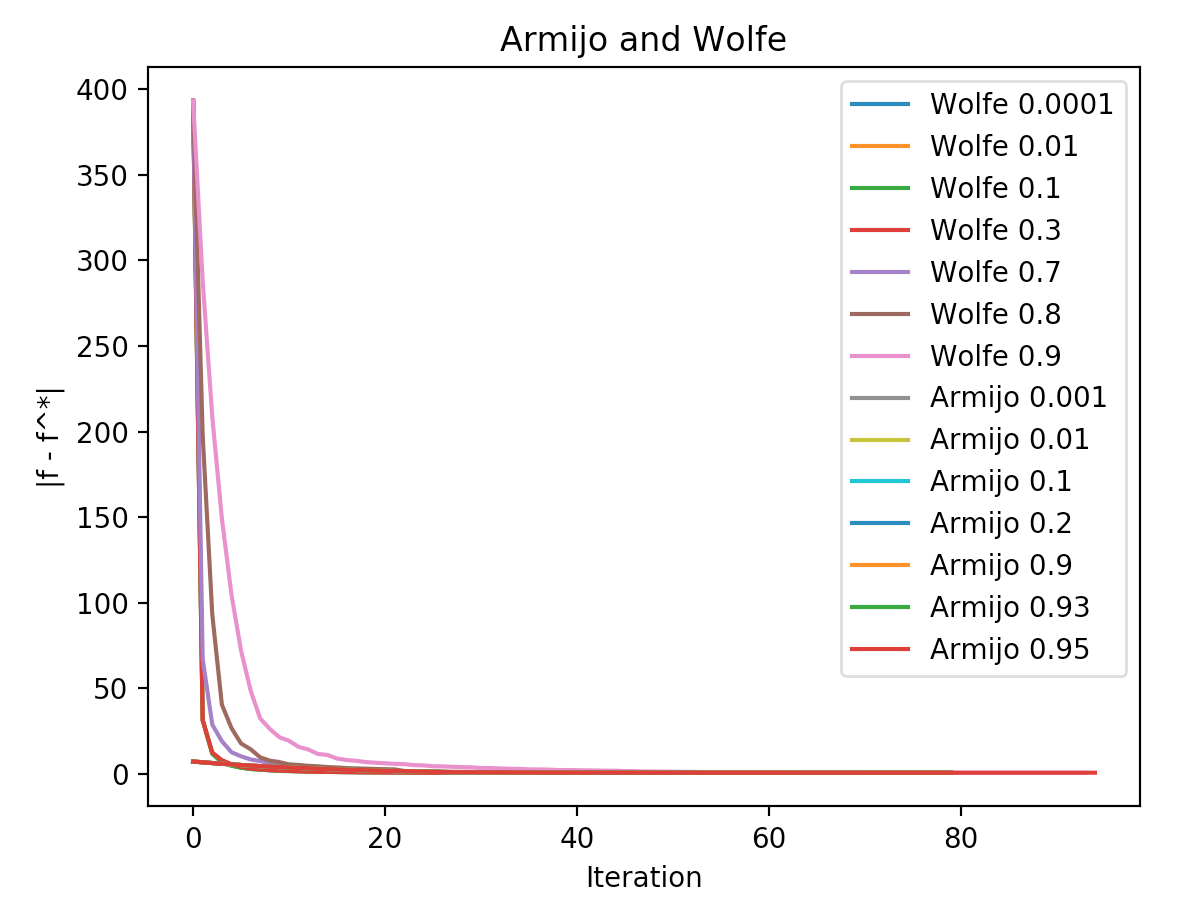
\includegraphics[width=0.6 \textwidth]{52.png}


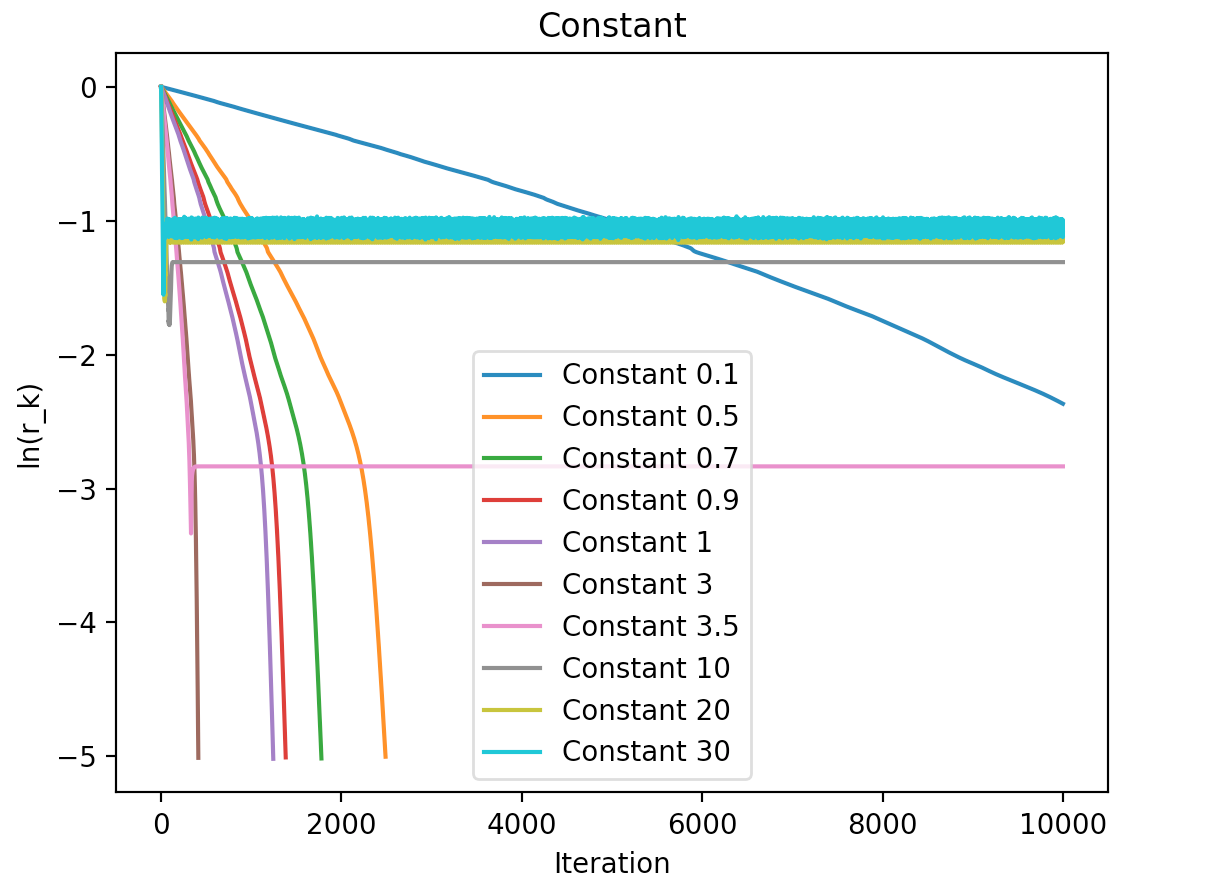
\includegraphics[width=0.6 \textwidth]{53.png}
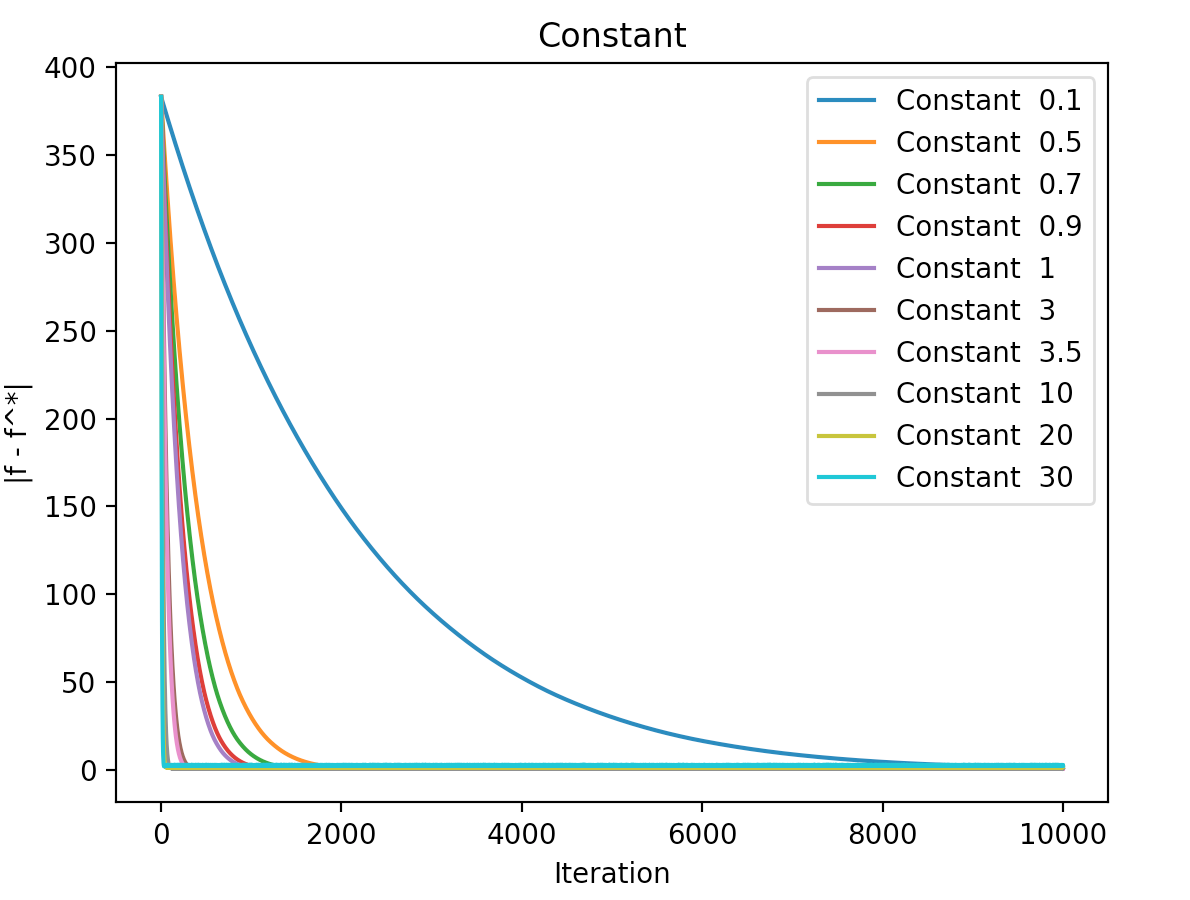
\includegraphics[width=0.6 \textwidth]{54.png}


Стратегия выбора длины шага в методе ньютона

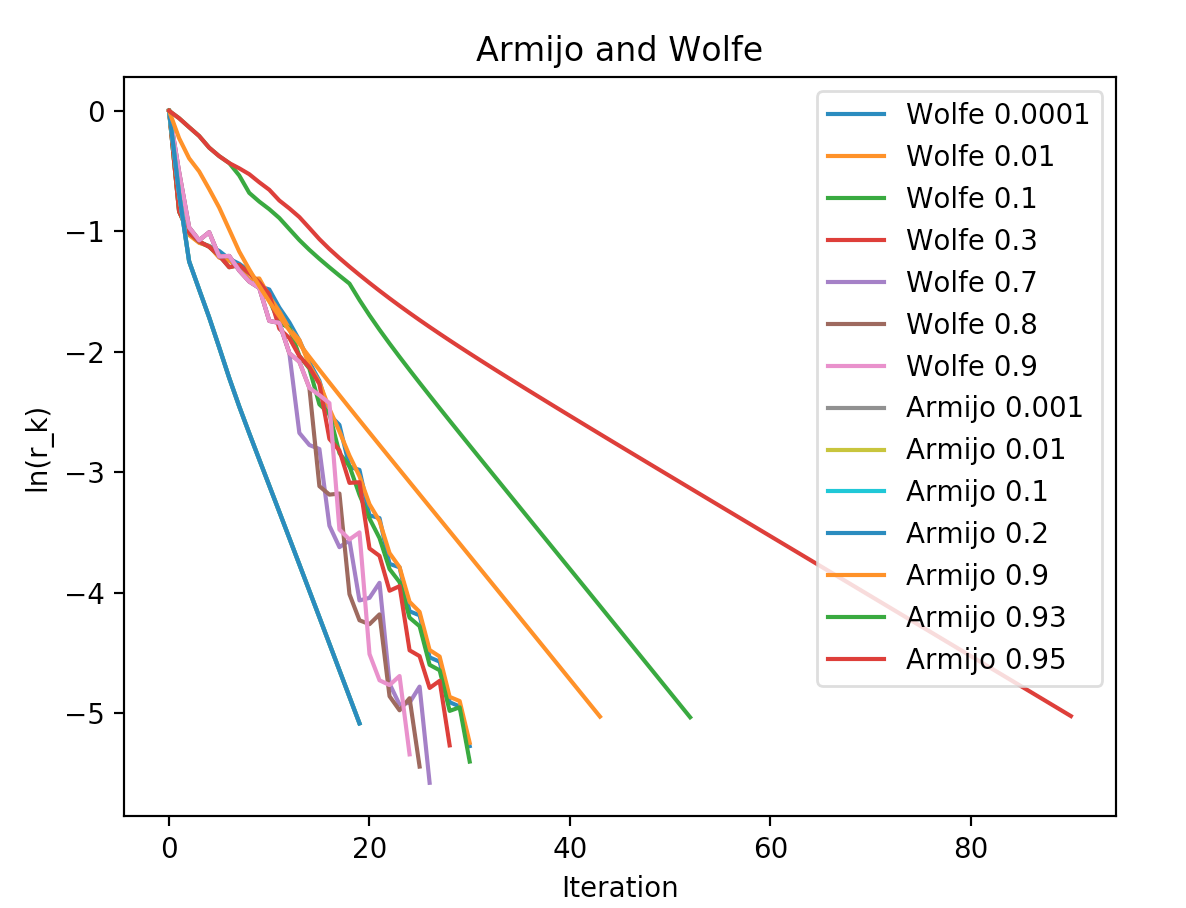
\includegraphics[width=0.6 \textwidth]{61.png}
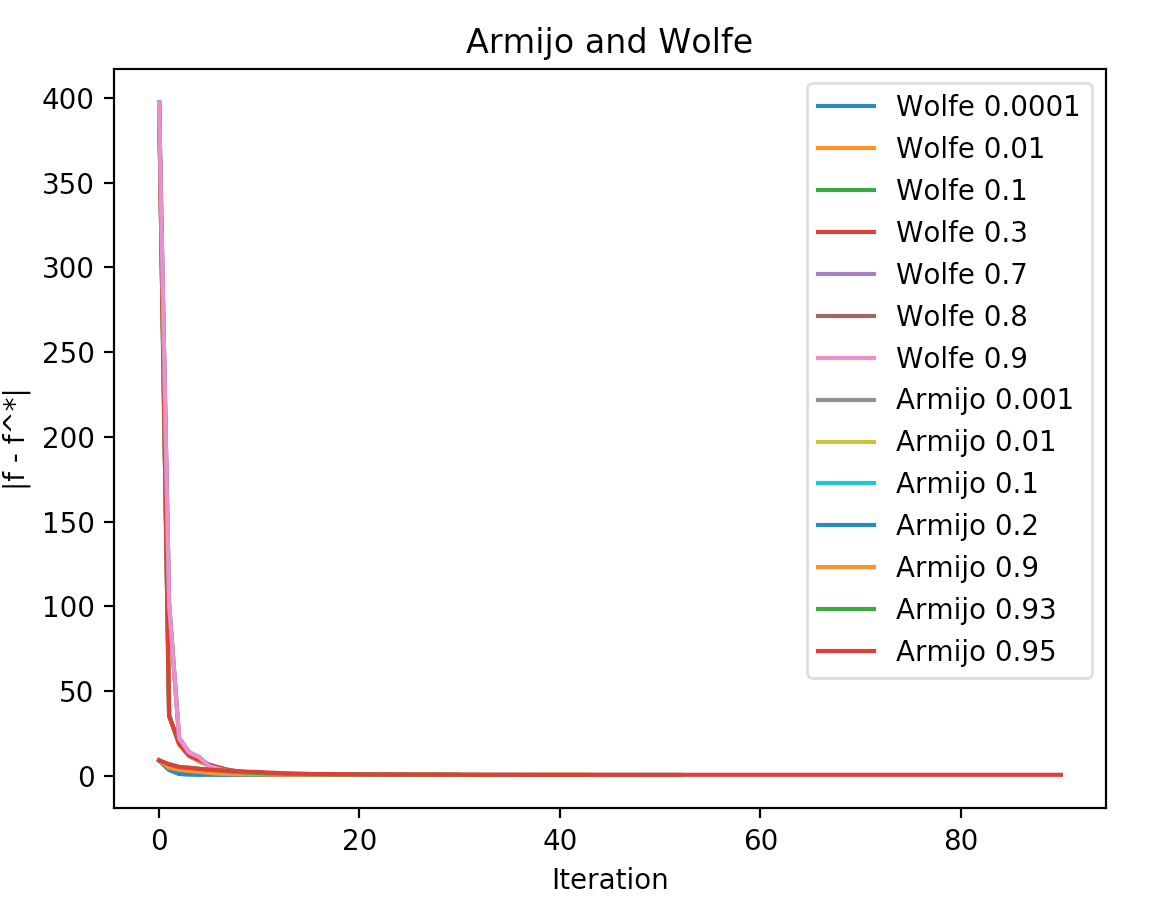
\includegraphics[width=0.6 \textwidth]{62.png}


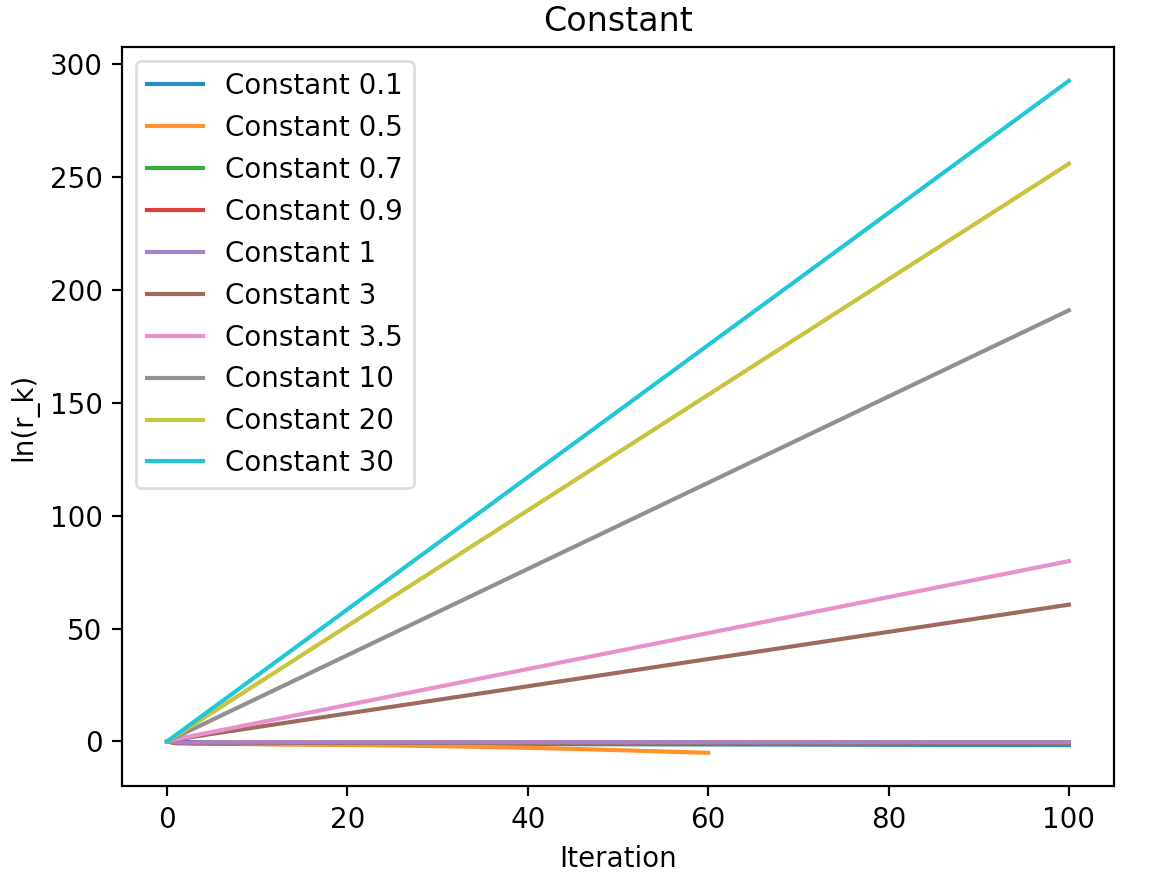
\includegraphics[width=0.6 \textwidth]{63.png}
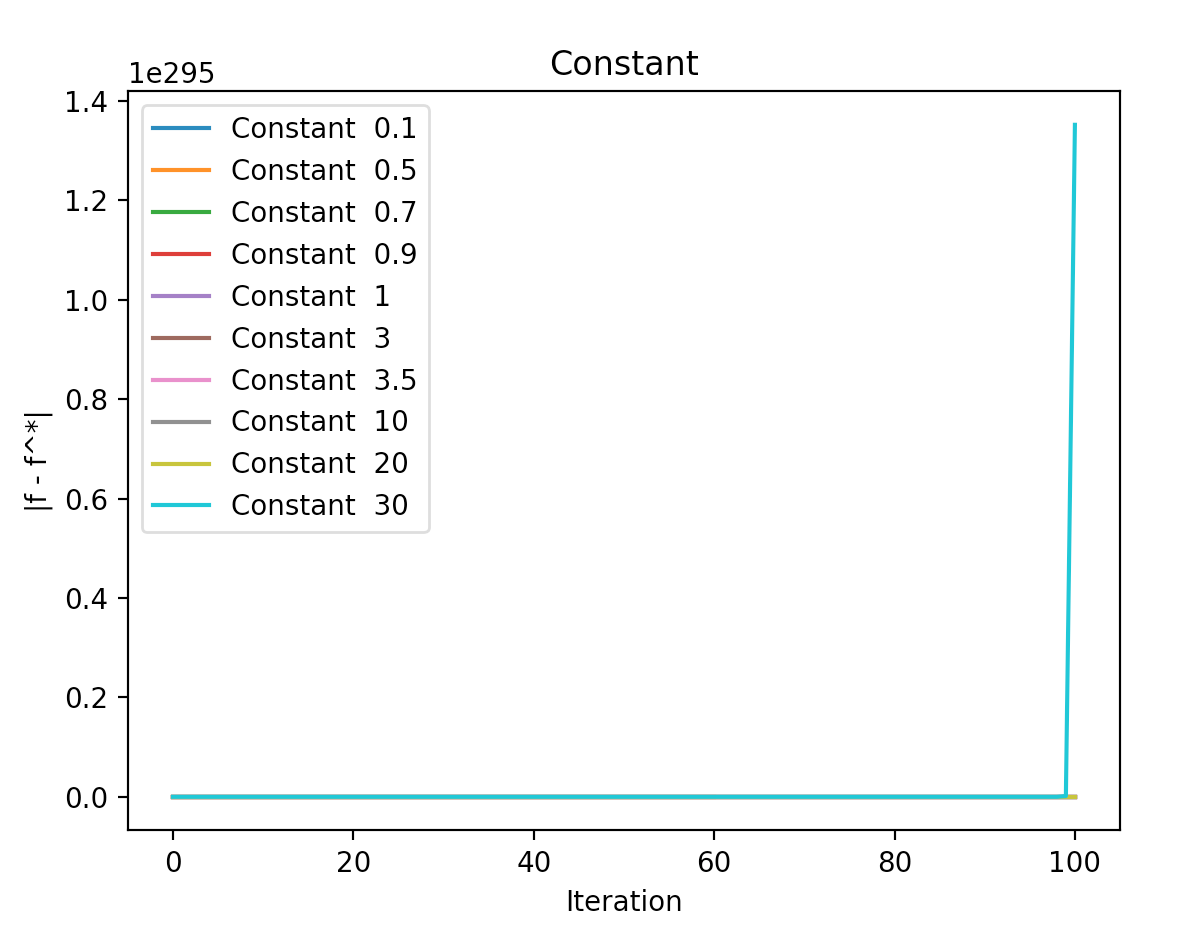
\includegraphics[width=0.6 \textwidth]{64.png}


\end{document}
